\documentclass[10.5pt,a4paper, fleqn, dvipsnames]{article}
\usepackage[utf8]{inputenc}
\usepackage[T1]{fontenc}
\usepackage{tikz}
\usetikzlibrary{shapes,positioning,arrows,fit,calc,graphs,graphs.standard}
% \usepackage[nosf]{kpfonts}
% \usepackage[t1]{sourcesanspro}
\usepackage[qcs]{tgschola}
\usepackage{multicol}
\usepackage{wrapfig}
\usepackage[top=0.8cm,bottom=0.8cm,left=0.75cm,right=1cm]{geometry}
% \usepackage[framemethod=tikz]{mdframed}
\usepackage{microtype}
\usepackage{pdfpages}
\usepackage{graphicx}

\usepackage{enumitem}
\setlist{nolistsep, leftmargin = 1em}
\setlist[2]{nolistsep, leftmargin = 1.5em}
% \setlist{nolistsep}
% \setlist{leftmargin = 1em}
\renewcommand{\labelitemii}{$\circ$}
\renewcommand{\labelitemiii}{$\rightarrow$}

\usepackage{xcolor}
% \usepackage[dvipsnames]{xcolor}
\definecolor{mygray}{rgb}{0.8,0.8,0.8}
\usepackage{listings}
\lstset{%
basicstyle=\ttfamily,
breaklines = true,
backgroundcolor=\color{mygray},
}
\usepackage{realboxes}
\usepackage{soul}
% \usepackage{amsthm,amsmath,amsfonts,amsthm,amstext,amssymb,fullpage,framed,fancybox,graphicx,color,mdwlist,pifont}
\usepackage{amsthm,amsmath,amsfonts,amsthm,amstext,amssymb}
\usepackage[hidelinks,bookmarks=true]{hyperref}
\usepackage[numbered]{bookmark}
\usepackage{lipsum}

\makeatletter
\newcommand*{\sectionbookmark}[1][]{%
  \bookmark[%
    level=section,%
    dest=\@currentHref,%
    #1%
  ]%
}
\makeatother



\begin{document}
\section*{Chapter 1 \& 2: Introduction and Decision Trees}
\sectionbookmark{Chapter 1 \& 2: Introduction and Decision Trees}
\begin{itemize}
    \item types of machine learning
    \begin{itemize}%[leftmargin = 1.2em]
        \item supervised machine learning: given a set of observations ($X$) and their corresponding targets ($y$), traing a model that relates $X$ to $y$ to predict new $X$s
        \item unsupervised machine learning: train a model to find patterns in a dataset (typically an unlabled one), an example would be clustering 
        \item Recommendation systems: predict the "rating" or "preference" a user would give to an item
    \end{itemize}
    \item classification vs regression:
    \begin{itemize}%[leftmargin = 1.2em]
        \item classification: predicting among two or more discrete classes
        \item regression: predicting a continuous value
    \end{itemize}
    \item we use baselines as a sanity check 
    \item \ul{Decision Trees}:
    \begin{itemize}%[leftmargin = 1.2em]
        \item are models that make prediction by sequentially look at features and checking if they're above/below a threshold
        \item each node represents a question or answer. The leaf nodes represent answers 
        \item fit looks to minimize impurity at each question (using the gini index)
        \item it considers all features at a particular node and decide which one is the most "important" to split on
        \item can be used for continous values (so regression) - use MSE instead of gini index
        \item hyperparameter: \lstinline!max_depth! $\rightarrow$ correlates with decision boundaries
    \end{itemize}
\end{itemize}
\section*{Chapter 3: ML Fundamentals}
\sectionbookmark{Chapter 3: ML Fundamentals}
\begin{itemize}
    \item splitting data is done so we can test how well our model is doing
    \begin{itemize}
        \item there's test and train set for training and testing (want to use test set once to evaluate performance of best performing model on validation set)
        \item there' also validation data for hyperparameter tuning
    \end{itemize}
    \item cross validation runs validation many time and give each fold a chance to be the validation set, avoid the scenario where you end up with a split that doesn't align/well represent your data
    \begin{itemize}
        \item advantage: Can assess model and reduce overfitting, can tune hyperparameter to get maximal performance
        \item disadvantage: Increase training time, and needs expensive computational power
    \end{itemize}\\
    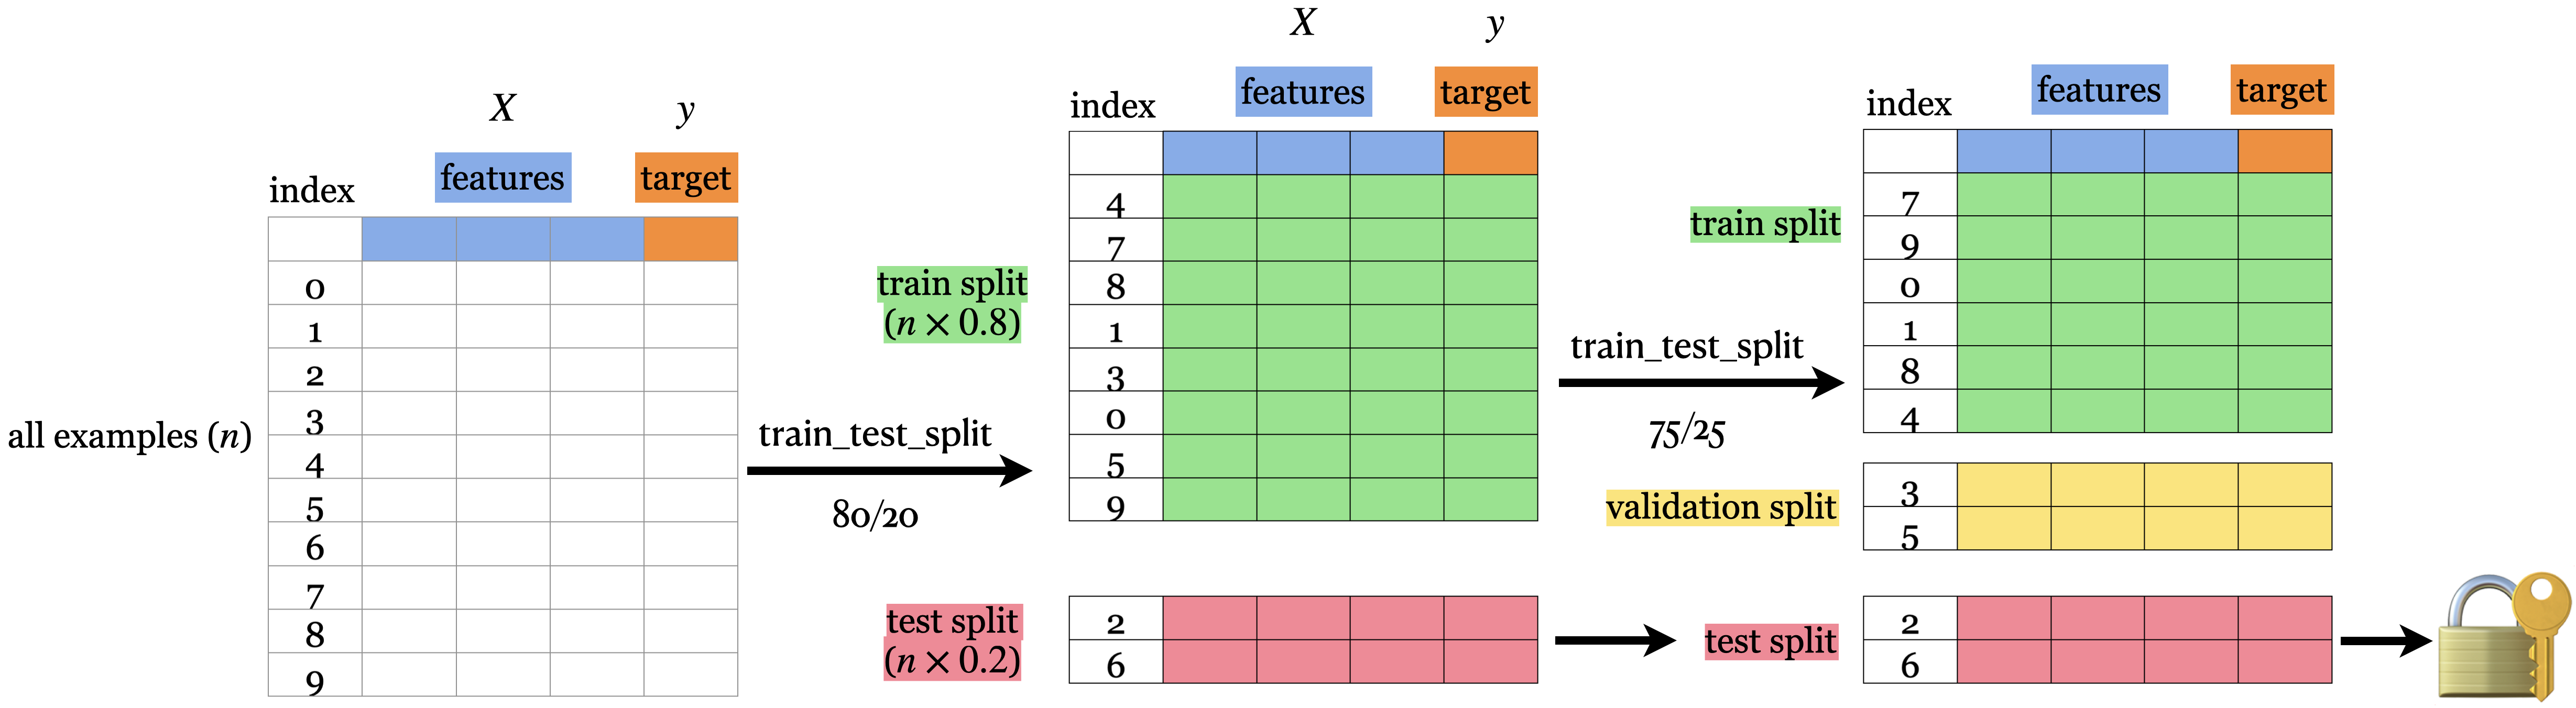
\includegraphics[scale = 0.2]{train-valid-test-split.png}
    \item overfitting: if model is very complex, then you'll learn unrealiable patterns to get every training example correct 
    \begin{itemize}[leftmargin = 1.2em]
        \item increasing complexity of models $=$ more chance of overfitting
        \item bad because the model is now resistant to new data
        \item sign: when training error is low but big gap between training error and validation error
    \end{itemize}
    \item undefitting: the model isn't learning/performing well enough on training data
    \item we want the model to be generalize-able to unseen data
    \item there are no perfect way to pick a hyper-parameter but \ul{most common way is to pick model with minimum cross-validation error (or highest cross-validation accuracy score)}
    \item \textbf{golden rule}: test data cannot influence training phase in any way
\end{itemize}

\section*{Chapter 4: $k$-NNs \& SVM-RBF}
\sectionbookmark{Chapter 4: $k$-NNs \& SVM-RBF}
\begin{itemize}
    \item k-Nearest Neighbours: 
    \begin{itemize}
        \item given some data points and their classes, we plot the data points and categorize them by colours or smt. Given a new data point, we grab the $k$ nearest neighbour (via Eucledian distance) and see the majority class
        \item \# of features = d-dimensions
        \item hyperparameter: \lstinline!n_neighbors! $\rightarrow$ how many closest points do wen consider
        \begin{itemize}[leftmargin = 2em]
            \item increasing \lstinline!n_neighbors! increases model complexity (overfitting)
        \end{itemize}
        \item most of the work is done during the \lstinline!predict! stage (rather than the \lstinline!fit! stage
        \item kNN is very bad with big number of dimensions, as well as when there are irrelevant attributes
    \end{itemize}
    \item parametric vs non-parametric:
    \begin{itemize}
        \item an algorithm is non-parametric if it needs to store $O(n)$ worth of stuff to make predictions
        \item parametric: \textbf{linear} SVM RBF
        \item non-parametric: $k$-NN is non-parametric (stores every data point to do distance calculations during \lstinline!predict!) 
        \begin{itemize}[leftmargin=2em]
            \item SVM RBF is also non-parametric
        \end{itemize}
    \end{itemize}
    \item SVM-RBF: another popular similarity-based algorithm 
    \begin{itemize}
        \item they're like weighted kNN
        \item decision boundary is defined by a set of positive and negative examples and their weights
        \item unlike kNN, SVM RBF only remember the key examples (support vectors) - so runs faster
        \item usually perform better too
        \item hyperparameter: \lstinline!gamma! and \lstinline!V!
        \begin{itemize}[leftmargin = 2em]
            \item larger \lstinline!gamma! = more complex 
            \item larger \lstinline!C! = more complex as well
        \end{itemize}
    \end{itemize}
    \item both kNN and SVM RBF has a regressor counterpart 
\end{itemize}

\section*{Chapter 5: Preprocessing Pipelines}
\sectionbookmark{Chapter 5: Preprocessing Pipelines}
\begin{itemize}
    \item when working with numeric data on different scales, and as a result features with larger values (scale) tends to dominate and smaller scale features get ignored
    \begin{itemize}
        \item we use a transformer: \lstinline!StandardScaler!
    \end{itemize}
    \item \lstinline!fit! and \lstinline!transform! paradigm
    \begin{itemize}
        \item \ul{split the data before you do pre-processing}
        \item \lstinline!fit_transform! the transformer on training set
        \item call \lstinline!transform! (only) on the test set
    \end{itemize}
    \item \ul{imputation}: tackle missing values 
    \begin{itemize}
        \item \lstinline!SimpleImputer! is the transformer we'll use 
        \item common strategy is to replace missing values with most frequent value in the categorical columns, and fill in the median value in the numeric columns 
    \end{itemize}
    \item \ul{one-hot encoding (OHE)}: tackle categorical values 
    \begin{itemize}
        \item we can transform categorical features into numeric ones so we can use them (assign an integer to each unique categorical label)
        \item \lstinline!OneHotEncoder! creates binary columns to represent our categories ($c$ categories in column results in $c$ new binary columns)
        \item \lstinline{handle_unknown = "ignore"} parameter gets it to ignore unknown value (happens when you have a low number of a category and it ends up in validation set and none in the training set - see Chapter 6 $\rightarrow$ dealing with unknown categories 
        \item \lstinline{drop = 'if binary'} is used for binary categories, it'll create 1 column of 0s and 1s instead of make 2 columns 
    \end{itemize}
    \item \ul{ordinal encoding}: when there is an order to the cateogrical features
    \begin{itemize}
        \item ex. Excellent $\rightarrow$ Good $\rightarrow$ Average $\rightarrow$ Poor
        \item see code in Chapter 6 $\rightarrow$ incorporating ordinal features 
        \item when you have more than one ordinal columns, you can pass a list of lists to \lstinline{OrdinalEncoder} where the inner list corresponds to the ordered cateogries for corresponding ordinal column (ex. \lstinline{[[Great, Okay, Bad], [Smart, Average, Stupid]]}
        \item whether you go best to worst or worst to best doesn't matter
    \end{itemize}
    \item to do pre-processing and CV and not break the golden rule, you're gonna need pipelines
    \begin{itemize}
        \item you can call \lstinline!fit! on the pipeline and it'll run through all the steps for you 
        \item can also call \lstinline!predict!
    \end{itemize}
\end{itemize}

\section*{Chapter 6: Column Transformer and Text Features}
\sectionbookmark{Chapter 6: Column Transformer and Text Features}
\subsection*{Column Transformers}
\begin{itemize}
    \item use \lstinline{ColumnTransformer} when you want to apply different transformers to different rows 
    \begin{itemize}
        \item i.e scaling for numeric features and OHE for cateogrical features
    \end{itemize}
    \item call \lstinline{fit_transform} on the training set
    \item you can pass column transformers into pipelines 
    \item after transforming data you might get a different size data sets\\
    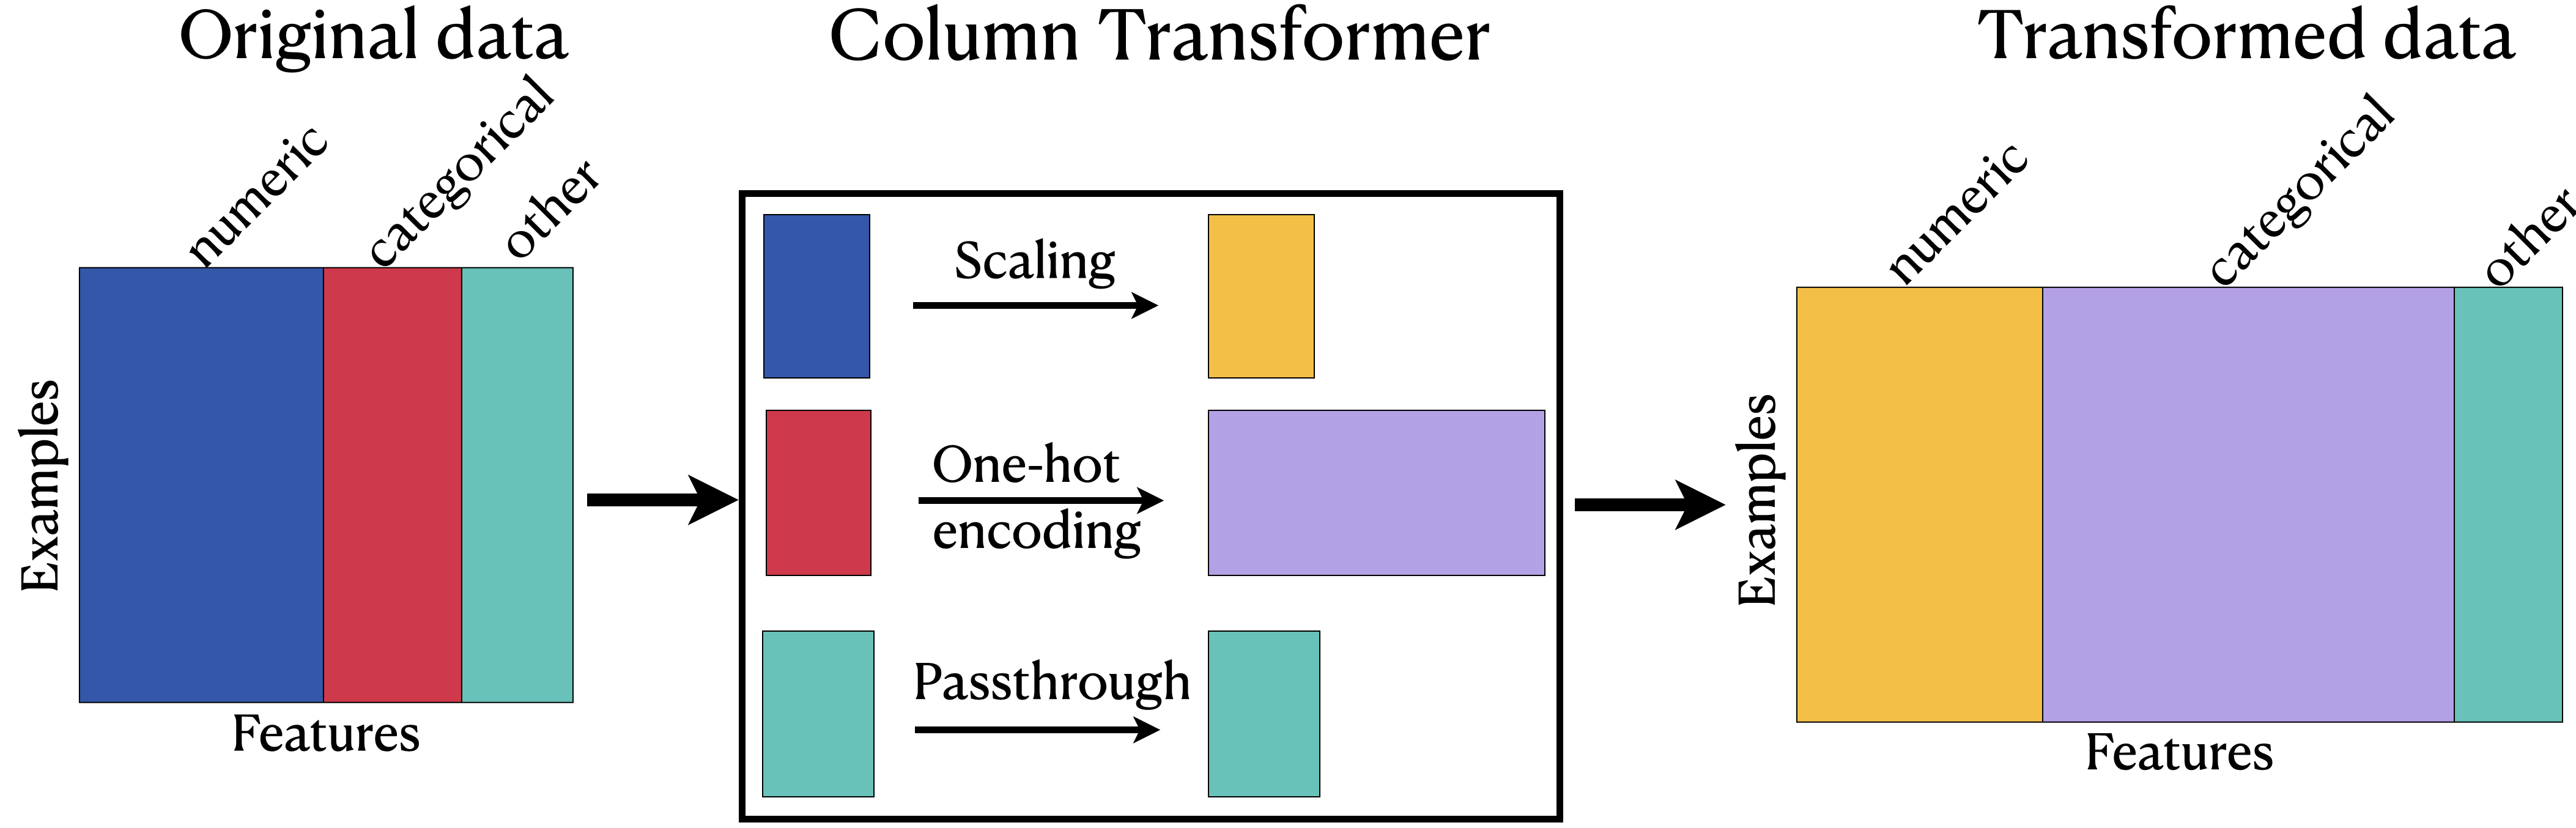
\includegraphics[scale = 0.18]{column-transformer.png}
    \begin{itemize}
        \item ex. \lstinline{pipe = make_pipeline(ct, SVC())}
    \end{itemize}
\end{itemize}
\subsection*{Encoding Text Features}
\begin{itemize}
    \item BOW representations 
    \begin{itemize}
        \item ignores the syntax and word order
        \item 2 components
        \begin{itemize}[leftmargin = 2em]
            \item the vocabs (all unique words in the documents)
            \item value indicating either the presence/absence or the count of each word in the document 
        \end{itemize}
        \item with CountVectorizer you need to define separate CountVectorizer transformers for each text column , if you have more than one text columns.
        \item see lecture 6 for hyper-parameters
    \end{itemize}
\end{itemize}

\section*{Chapter 7: Linear Models}
\sectionbookmark{Chapter 7: Linear Models}
\begin{itemize}
    \item linear models is a fundamental and widely used class of models. They are called linear because they make a prediction using a linear function of the input features
    \item \ul{Linear regression}
    \begin{itemize}
        \item each feature is assigned a coefficient and the model learns an intercept, given new data points, you can plug in the multiply by the weights and add them up for the prediction
        \item when we call \lstinline{fit}, a coefficient/weight is learned for each features and they're learned from the training data 
        \begin{itemize}[leftmargin = 2em]
            \item positive coefficient means proportional: bigger feature = bigger target 
            \item magnitude: bigger magnitude means bigger impact on prediction 
            \item when interpreting coefficients, scaling is crucial 
        \end{itemize}
        \item in linear models for regression, the model is a line for a single feature, a plane for two features, and a hyperplane for higher dimensions $\rightarrow$ so we'll have a $k$-dimensional plane for $k$ features
    \end{itemize}
    \item \ul{Ridge}
    \begin{itemize}
        \item is another linear regression model with a complexity hyper-parameter \lstinline{alpha}
        \item bigger \lstinline{alpha} means underfitting (alpha being 0 is the same as using Linear Regression)
    \end{itemize}
    \item \ul{Logistic Regrssion}
    \begin{itemize} 
        \item \ul{\textbf{is a linear model for classification}}
        \item it outputs a raw score, and based on a threshold (i.e raw score > 0.50), it will decide on whether the class is positive or negative 
        \begin{itemize}[leftmargin = 2em]
            \item raw score below the threshold would be predicted as a negative class
        \end{itemize}
        \item also has coefficients (interpretation is similar to linear regression)
        \item model usually randomly considers one class to be "positive" or "negative"
        \begin{itemize}[leftmargin = 2em]
            \item \lstinline{classes_} attribute tells us which class is considered negative and positive 
            \item is off the form [negative, positive]
        \end{itemize}
        \item hyperparamter: \lstinline{C} - bigger C means overfitting 
    \end{itemize}
    \item \lstinline{predict_proba} 
    \begin{itemize}
        \item is a soft prediction, i.e how confident a model is with a given prediction 
        \item you can call \lstinline{predict_proba} and it'll give you [probability it's the negative class, probability it's the positive class]
        \item these values are achieved by feeding the raw score (weighted sum) into the sigmoid function 
        \item points closer to the boundary means model is less confident 
    \end{itemize}
    \item see chapter 7 on using LR with words 
\end{itemize}

\section*{Chapter 8: Hyperparameter Optimization and Optimization Bias}
\sectionbookmark{Chapter 8: Hyperparameter Optimization and Optimization Bias}
\subsection*{Hyperparameter Optimization}
\begin{itemize}
    \item manual hypereparmter optimization like we've been doing takes a lot of work, not reproducible, and in complicate cases (i.e multiple hyper parameter) $\rightarrow$ intuition might be worse 
    \item \lstinline{GridSearchCV}: 
    \begin{itemize}
        \item we need
        \begin{itemize}[leftmargin = 2em]
            \item instatianted model or pipeline
            \item parameter grid: user specified set of values for each hyperparameter that we're gonna look through
            \item other optional argument (i.e \lstinline{n_jobs = -1} which means use all cores)
        \end{itemize}
        \item the method considers every combination of the value sets and test out each one 
        \item you can call \lstinline{fit}, \lstinline{predict}, or \lstinline{score} on it and call \lstinline{best_score_} and \lstinline{best_params_} attributes 
        \item the range of which we pick the hyperparameter to be in play an important results 
        \item \textbf{\ul{computation}}: if you have 5 hyperparameters, and 10 different values for each hyperparameters, you will have to evaluate $10^5$ models (not counting number of cv folds)
    \end{itemize}
    \item \lstinline{Randomized Hyperparameter Search}
    \begin{itemize}
        \item you specified a list of values for each hyperparmeter, similar to above
        \item difference is this one picks random combinations to try out
        \item hyperparameter: \lstinline{n_iter} tells it how many models to try out
    \end{itemize}
    \item note that the exponential range for the hyperparameter \lstinline{C} is quite common (usually $10^n$ where $n = -2, -1, 0, 1, 2, \ldots$)
    \item advantages of \lstinline{Randomized Hyperparameter Search}
\end{itemize}
\subsection*{Optimization bias/Overfitting of the validation set}
\begin{itemize}
    \item when our dataset is small and if your validation set is hit too many times, we suffer from optimzation bias or overfitting of the validation set 
    \item optimization bias of parameter learning 
    \begin{itemize}
        \item basically overfitting with training error
    \end{itemize}
    \item optimization bias:
    \begin{itemize}
        \item when training data is small and so is the validation splits, we could hit the same validation set many times and that validation might have given us good results 
        \begin{itemize}[leftmargin = 2em]
            \item so like the the small validation set could have just been really good but this model keeps using it over and over so we keep getting this great score over and over
        \end{itemize}
        \item even though validation splits will not influence training directly - it will influence hyperparameter optimzation
    \end{itemize}
    \item so we can trust validation scores when the training data is of good size, and we can trust the test score score when the test set is of good size 
\end{itemize}

\section*{Chapter 9: Classification Evaluation Metrics}
\sectionbookmark{Chapter 9: Classification Evaluation Metrics}
\begin{itemize}
    \item when we have an unbalanced dataset, accuracy will not be a good metrics 
    \item when we're trying to spot a certain label (i.e fraud) $\rightarrow$ this is called the positive class
    \item confusion matrix
    \begin{itemize}
        \item false positives (type 1 errors): model incorrectly spots examples as fraud
        \item false negatives (type II errors): it didn't classify fraud examples as fraud (classified them non-fraud instead) 
        \item diagonal entries are the perfect predictions while the off diagonals tell us what is being mis-interpreted
        \item note that the order of the cells could be different sometimes (though the diagonal thing is always true)\\
        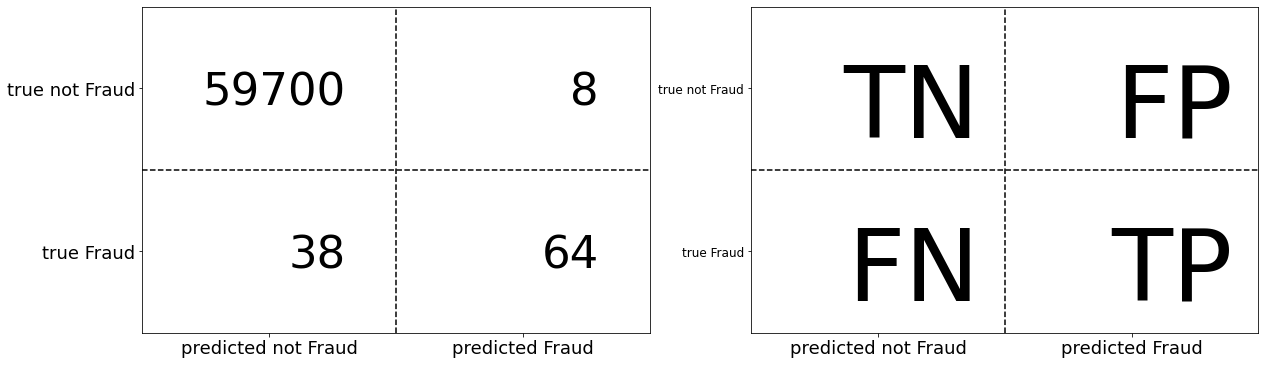
\includegraphics[scale = 0.35]{confusion-matrix.png}
    \end{itemize}
    \item other scoring metrics for when there's a class imbalance and we can't use accuracy
    \begin{itemize}
        \item recall: among all positive examples, how many did you identify
        \begin{align*}
            recall = \dfrac{TP}{TP + FN} = \dfrac{TP}{\text{\# of positives}}
        \end{align*}
        \item precision: among the positive examples you identified, how many were actually positive?
        \begin{align*}
            precision = \dfrac{TP}{TP + FP}
        \end{align*}
        \item f1-score: combines precision and recall to give one score - good for hyperparameter optimization
        \begin{align*}
            f1 = 2 \times \dfrac{\text{precision} \times \text{recall}}{\text{precision} + \text{recall}}
        \end{align*}
        \item you can use \lstinline{classification_report} to get this, the rows are "what if this class was the positive class" \\
    \end{itemize}
    \item \textbf{when you're trying to avoid false-negatives: use recall}
    \begin{itemize}
        \item ex. false negatives are very bad in cancer diagnosis - we'd rather falsely diagnose someone and give them tests than to let them go when they have cancer
    \end{itemize}
    \item \textbf{when cost of a false-positive is high: use precision}
    \begin{itemize}
        \item ex. you're a restaurant looking to buy wine only if it's been predicted as good by a classifier - since cost is limited, we don't want to waste money on shitty wine, we rather miss out on some good wines but all the ones we buy to be good
    \end{itemize}
    \item accuracy and these new metrics are not very correlated (i.e model A having higher accuracy than model B doesn't mean it has higher precision) - \ul{there is a relationship between precision and recall however}
    \item \ul{operating point}: confusion matrix uses hard predictions, here we're leveraging the confidence (\lstinline{predict_proba}) of the model to understand the model performance
    \begin{itemize}
        \item if you want to achieve a certain percentage for the "fraud class", you can change the threshold of \lstinline{predict_proba} (so you can make it smaller to identify more positive examples)
        \item setting a requirement on a classifier (e.g recall of >= 0.75) is called setting the \textbf{operating point}
    \end{itemize}
    \newpage
    \item precision/recall tradeoff
    \begin{itemize}
        \item there's a trade off between precision and recall
        \item if you identify more things as "fraud", recall is going to increase but there are likely to be more false positives 
        \item decreasing the threshold means lower bar for predicting fraud
        \begin{itemize}
            \item you are willing to risk more false positives in exchange of more true positives.
            \item recall would either stay the same or go up and precision is likely to go down
            \item \ul{point: decreasing threshold likely to increase recall and decrease precision}
        \end{itemize}
        \item increasing the threshold means a higher bar for predicting fraud
        \begin{itemize}
            \item recall would go down or stay the same but precision is likely to go up
            \item occasionally, precision may go down as the denominator for precision is TP+FP.
            \item \ul{point: increasing the threshold usually means recall goes down and precision goes up}
        \end{itemize}
    \end{itemize}
    \item \ul{PR (precision-recall) Curve} \\
    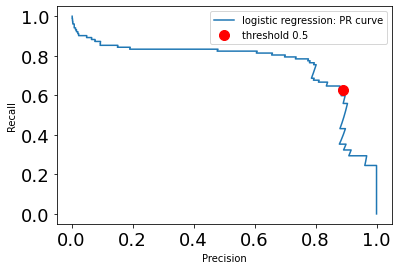
\includegraphics[scale = 0.65]{pr-curve.png}
    \begin{itemize}
        \item the red dot correspond to the threshold we specified for the \lstinline{predict_proba}
        \begin{itemize}[leftmargin = 2em]
            \item so, we can achieve a recall of 0.8 and precision of 0.4 when the threshold is 0.5
            \item here we have a high precision but lower recall.
            \item usually goal is to keep recall high as precision goes up
        \end{itemize}
        \item AP score: is a number to summarize the PR plot
        \begin{itemize}[leftmargin = 2em]
            \item AP (average precision) score: area under the PR curve
            \item has value from 0 (worst) to 1 (best)
        \end{itemize}
    \end{itemize}
    \item AP vs F1 score
    \begin{itemize}
        \item F1 score is for a given threshold and measures the quality of predict. (default uses threshold \lstinline{predict_proba > 0.5})
        \item AP score is a summary across thresholds and measures the quality of \lstinline{predict_proba}.
    \end{itemize}
    \item \ul{ROC curve}
    \begin{itemize}
        \item another commonly used tool to analyze the behavior of classifiers at different thresholds.
        \item similar to PR curve, it considers all possible thresholds for a given classifier given by \lstinline{predict_proba} but instead of precision and recall it plots false positive rate (FPR) and true positive rate (TPR or recall).
        \begin{align*}
            FPR = \dfrac{FP}{TN + FP} ~~~~~~~ TPR = \dfrac{TP}{TP+FP}
        \end{align*}
        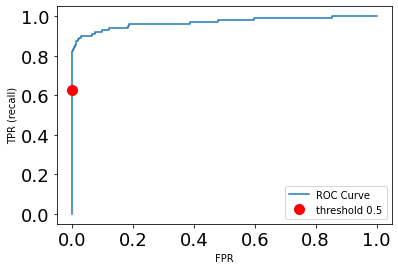
\includegraphics[scale = 0.65]{roc-curve.png}
        \begin{itemize}
            \item ideal curve is to the top left (classifier with high recall while keep low FPR)
            \item the red dot correspond the threshold of 0.5
        \end{itemize}
        \item AUC (area under the curve): provides a meaningful number for model performance (based on ROC curve)
        \begin{itemize}[leftmargin = 2em]
            \item AUC of 0.5 means random chance 
        \end{itemize}
    \end{itemize}
    \item for classification problems w/ imbalanced classes, AP score or AUC is often much more meaningful than accuracy
    \item handling imbalance: in this class we'll look into handling imbalances using weighs (\lstinline{class_weights} in sklearn)
    \begin{itemize}
        \item \lstinline{class_weight}= balance reduces false negatives but increases false positives higher recall but lower precision
       \item \lstinline!class_weight = {x: y}! reduces false negatives but increases false positives also
    \end{itemize}
    \newpage 
    \item summary:
\end{itemize}
    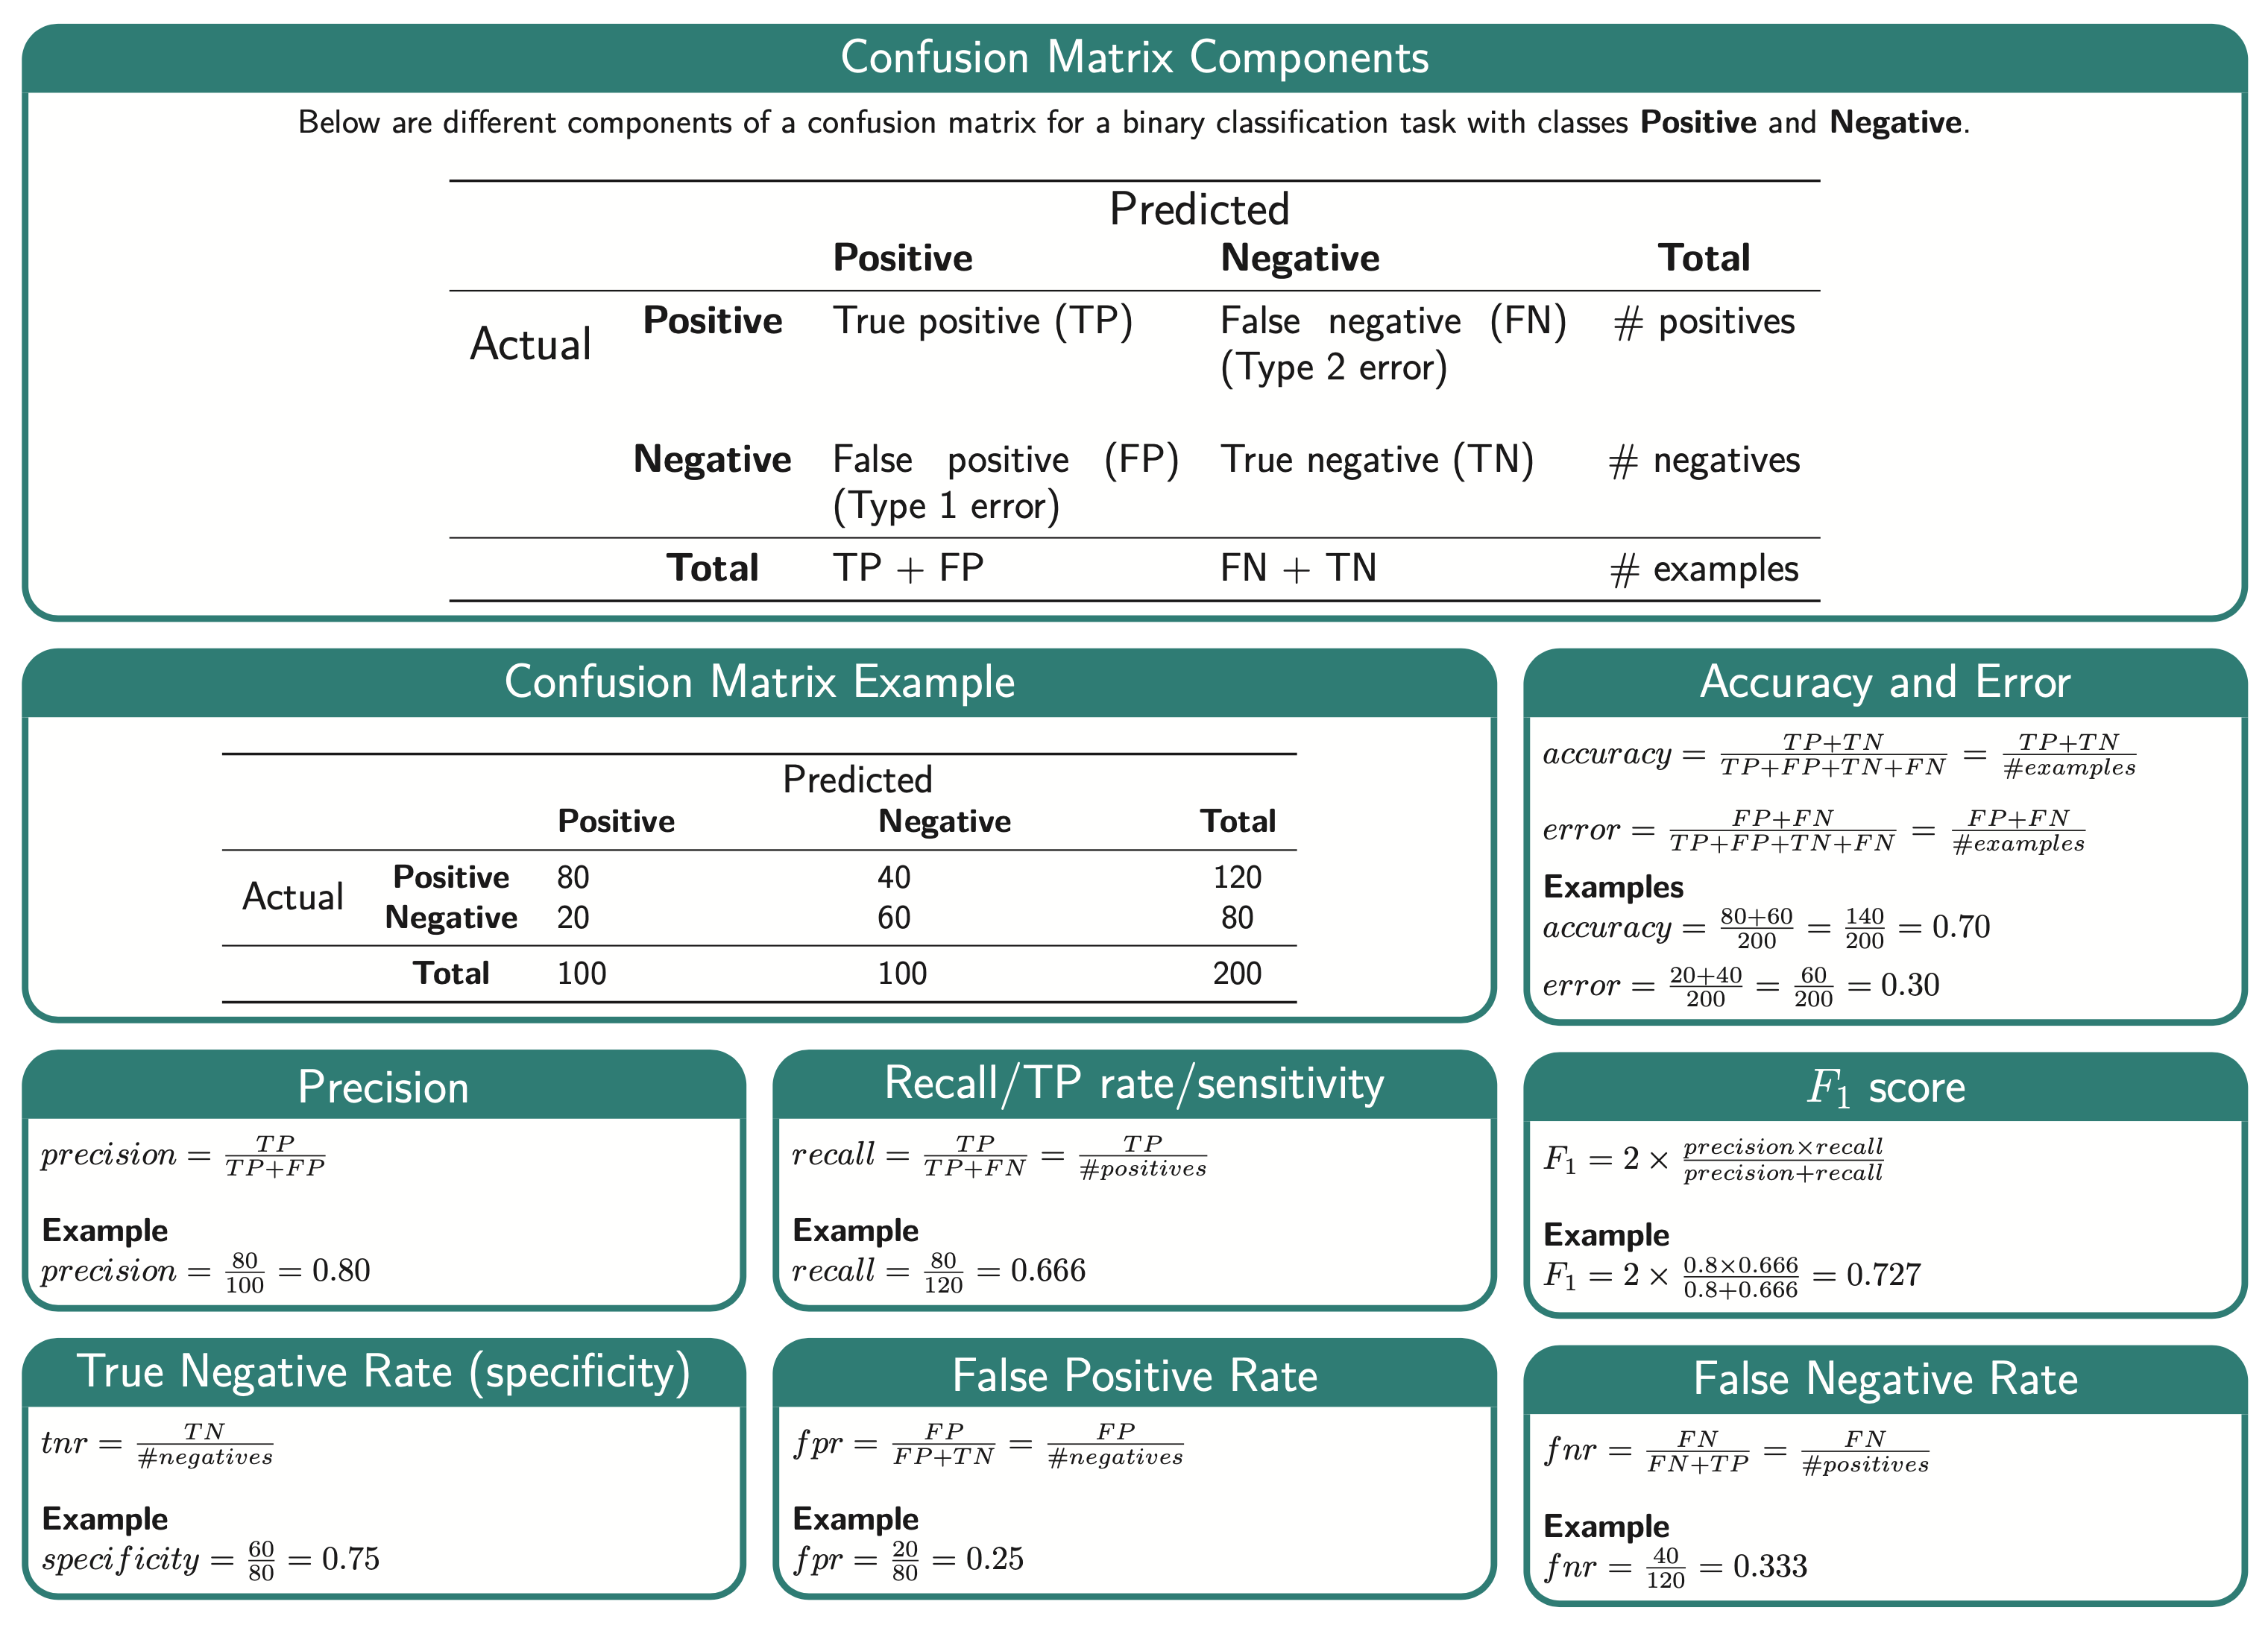
\includegraphics[scale = 0.37]{evaluation-metrics.png}

\section*{Chapter 10: Regression Evaluation Metrics}
\sectionbookmark{Chapter 10: Regression Evaluation Metrics}
\begin{itemize}
    \item beginning of chapter 10 has quite a nice workflow if you need to see code
    \item regression score functions: since we're not doing classification anymmore, we cna't just check for equality, some common metrics are
    \begin{itemize}
        \item mean squared error (MSE)
        \item $R^2$
        \item roote mean squared error (RMSE)
        \item MAPE
    \end{itemize}
    \item \ul{mean square error (MSE)}
    \begin{itemize}
        \item perfect predictions have MSE = 0
        \item the score depends on the scale of our targets (and units) - so scores can get a big an unwieldy
        \item also, the unit of the score is different (target is in dollars, MSE is in $\text{dollar}^2$)
    \end{itemize}
    \item \ul{root mean square errors (RMSE)}
    \begin{itemize}
        \item a more relatable metric 
        \item is the square root of the MSE
    \end{itemize}
    \item \ul{$R^2$}
    \begin{itemize}
        \item is used by default by sklearn when you call \lstinline{score()}
        \item max value is 1 (for perfect predictions)
        \item values can be negative (worse than dummy regressor - very bad)
        \item sklearn uses the negative version of this (negative root mean squared error), and it does this because it wants to think of it in the context of maximizing (so higher neg RMSE is better)
    \end{itemize}
    \item \ul{MAPE}
    \begin{itemize}
        \item takes into account the relative error (i.e 30k error for a 600k house is reasonable, but for a 60k house, it's awful)
        \item \ul{it looks at percent error} and takes the average over all examples
        \item ex. if we get MAPE score of 10.09, we can interpret as "on average, we have around 10\% error"
    \end{itemize}
    \item \textbf{\ul{transforming the target}}
    \begin{itemize}
        \item linear regression models by default try to minimize RMSE, but sometimes we'd like it to minimize MAPE
        \item common practice to get \lstinline{.fit()} to care about MAPE is to \ul{log transform the targets} - so $y \rightarrow \log(y)$
        \begin{itemize}
            \item \ul{we log transform when there are extreme values} and when we want interpretability in terms of units
        \end{itemize}
    \end{itemize}
    \item you can also use these scoring functions with \lstinline{cross_validate}, by passing them into the \lstinline{scoring = "(insert metric")}
\end{itemize}

\section*{Chapter 11: Ensembles}
\sectionbookmark{Chapter 11: Ensembles}
\begin{itemize}
    \item ensembles: models that combine multiple ML models to create more powerful models 
    \item tree-based ensemble models 
    \begin{itemize}
        \item decision trees are interpretable and can capture non-linear relationships, but likely to overfit $\rightarrow$ idea is to combine multiple trees to make a stronger model 
    \end{itemize}
    \item \lstinline{RandomForestClassfier}
    \begin{itemize}
        \item hyperparemter:
        \begin{itemize}[leftmargin = 2em]
            \item \lstinline{n_estimators}: tell it how many trees we want to build (higher = more complexity)
            \item \lstinline{max_depth}: max depth of each decision tree (higher = more complexity)
            \item \lstinline{max_features}: number of features to look at at each split (higher = more complexity)
        \end{itemize}
        \item \lstinline{fit} a diverse set of many decision trees by injecting randomness into the classifier construction 
        \item predicting by voting (classification) or averaging (regression) the predictions given by individal trees 
        \item injecting randomness:
        \begin{itemize}[leftmargin = 2em ]
            \item data: Build each tree on a bootstrap sample (i.e., a sample drawn with replacement from the training set
            \begin{itemize}
                \item ex. Suppose this is your original dataset: [1,2,3,4]\\
                a sample drawn with replacement: [1,1,3,4]\\
                a sample drawn with replacement: [3,2,2,2]\\
                a sample drawn with replacement: [1,2,4,4]
            \end{itemize}
            \item features: at each node, select a random subset of features (controlled by \lstinline{max_features} and we select new subset at every node) and look for the best split involving one of these features
        \end{itemize}
        \item ensembles seem to beat the fundamental tradeoff - we can increasing the training score while at the same time not decreasing validation score so much 
        \item pros:
        \begin{itemize}[leftmargin = 2em ]
            \item usually one of the best performing off-the-shelf classifiers without heavy tuning of hyperparameters
            \item don't require scaling of data - all tree based model not that sensitive to scale of data
            \item less likely to overfit
            \item In general, able to capture a much broader picture of the data compared to a single decision tree.
        \end{itemize}
        \item cons:
        \begin{itemize}[leftmargin = 2em]
            \item require more memory
            \item hard to interpret
            \item tend not to perform well on high dimensional sparse data such as text data
        \end{itemize}
    \end{itemize}
    \item Gradient Boosted Trees
    \begin{itemize}
        \item ex. \lstinline{XGBoost}, \lstinline{LightGBM}, \lstinline{CatBoost} 
        \item there are no randomization
        \item idea so to combine many simple models (weak learners) to create strong learners
        \item they combine multiple shallow (depth 1-5) decision trees 
        \item build trees in a serial manner, where each tree tries to correct mistakes of previous ones
        \item hyperparamter:
        \begin{itemize}[leftmargin = 2em]
            \item \lstinline{n_estimators}: number of trees to build
            \item \lstinline{learning_rate}: controls how strongly each tree tries to correct mistake of previous ones (higher learning rate = more complex models)
        \end{itemize}
    \end{itemize}
    \item which model to pick: pick the one that has the best CV score, but also take into consideration CPU cost
    \item \ul{Averaging}: use a bunch of models, predict for each example, and use the majority or average 
    \begin{itemize}
        \item uses \lstinline{VotingClassifier}
        \item as long as different models make different mistakes, this would work \\
        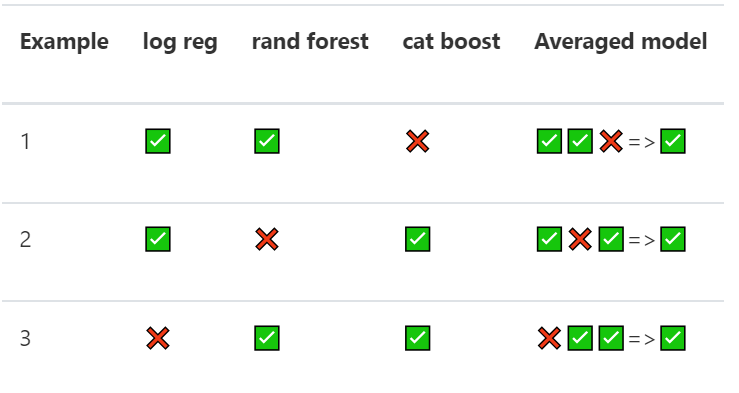
\includegraphics[scale = 0.52]{averaging-example.png}
        \item cons: 
        \begin{itemize}[leftmargin = 2em]
            \item takes a long time
            \item reduction in interpretability
            \item reduction in code maintainability 
        \end{itemize}
    \end{itemize}
    \item \ul{Stacking}: 
    \begin{itemize}
        \item instead of averaging the outputs of each estimator, we use their outputs as inputs to another model 
        \item the final estimator by default, for classification is logistic regression
        \begin{itemize}[leftmargin = 2em]
            \item it takes in predictions (\lstinline{predict_proba} scores) of other classifiers for each example
            \item so number of coefficients (and number of features) = number of base estimators 
        \end{itemize}
        \item the coefficients we get back from LR can be interpreted as which base model LR thought was the most important in predicting a class 
        \item usually takes longer than voting, but generally have higher accuracy (you can also see the coefficients)
    \end{itemize}
\end{itemize}

\section*{Chapter 12: Feature Importance}
\sectionbookmark{Chapter 12: Feature Importance}
\begin{itemize}
    \item during EDA, we can look at correlation between various features with other features and the target in our encoded data 
    \begin{itemize}
        \item see notebook to see how to call heat maps
        \item big positive values in cells mean $X$ and $Y$ is highly correlated
        \item this \ul{approach is too simplistic} though
        \begin{itemize}[leftmargin = 2em]
            \item only looks at features in isolation and linear associations 
            \item ex. \lstinline[language = python]{SalePrice} is deemed uncorrelated with \lstinline{BsmtFullBath} but it may be the case that \lstinline[language = python]{SalePrice} is high when \lstinline[language = python]{BsmtFullBath} is 2 or 3, but low when it's 0, 1 \textbf{or 4} (and hence it'll seem uncorrelated)
        \end{itemize}
        \item it can give us a good hint about high correlation - but don't take the uncorrelated measurements too seriously
    \end{itemize}
    \item interpretation of correlation 
    \begin{itemize}
        \item if $Y$ goes up when $X$ goes up, we say $X$ and $Y$ are positively correlated
        \item if $Y$ goes down when $X$ goes up, we say they're negatively correlated
        \item if $Y$ is unchanged when $X$, we say they're uncorrelated
    \end{itemize}
    \item \ul{feature importance in linear models}: for linear models (i.e logistic regression and linear regression, we can look at \ul{coefficients} for each features, let's look at how to interpret them
    \begin{itemize}
        \item \textbf{ordinal features}: how much the predicted target (i.e \lstinline{SalePrice}) increase/decrease by the feature (i.e \lstinline{ExteriorQuality} going up one category (i.e good $\rightarrow$ excellent)
        \item \textbf{categorical features}: each category gets their own coefficients, we can talk about the change in prediction from switching one to another by picking a "reference" category, and subtract everything by that
        \begin{itemize}[leftmargin = 2em]
            \begin{figure}[!h]
                \centering
                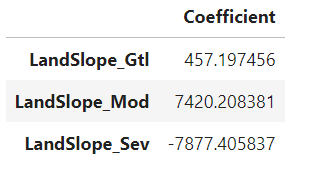
\includegraphics[scale = 0.85]{landslope coeff.png} 
                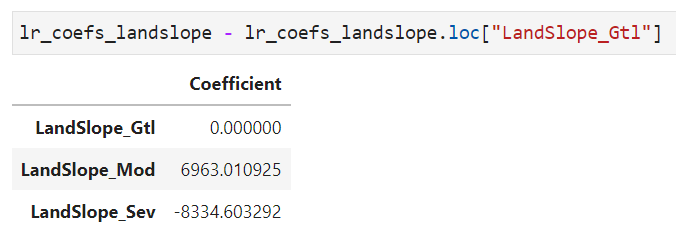
\includegraphics[scale = 0.75]{landslope coeff 2.png}
                \label{fig:my_label}
            \end{figure}
            \item ex. we have the following coefficients for the categories inside \lstinline{LandSlope}. This means that you change category from \lstinline{LandSlope_Gtl} to \lstinline{LandSlope_Mod} the prediction price goes but by \$6963 
        \end{itemize}
        \item numeric features: is tricky because numeric features are scaled (calling \lstinline{coefs} alone will get you weird numbers that might not be correct to scale)
        \begin{itemize}[leftmargin = 2em]
            \item we needed to access the scaler and unscale it
            \item once you do that, the coefficient that if we increase the \textbf{scaled} feature by one unit the price would go up $z$ amount 
        \end{itemize}
    \end{itemize}
    \item interpretability: ability to interpret ML models is important - we can leveraged by domain experts to diagnose systematic errors and underlying biases
    \begin{itemize}
        \item simple models are more interpretable but not as accurate 
    \end{itemize}
    \item interpretability and feature importance beyond linear models
    \begin{itemize}
        \item sklearn has package \lstinline{features_importances_} that gives feature importance for sklearn's tree based algorithms  
        \begin{itemize}[leftmargin = 2em]
            \item unlike linear model coefficients, \lstinline{features_importances_} doesn't have a sign 
            \item they tell us about importance (how important it is to the model's prediction) but not "up" or "down"
            \item because increasing a feature may cause prediction to go up, then down (not possible in linear models)
        \end{itemize}
        \item \ul{eli5}: used to get feature importance for non sklearn models - you get feature importance coefficients just like you would for sklearn's model
        \item \ul{SHAP}: sophisticated measure of contribution of each feature 
        \begin{itemize}[leftmargin = 2em]
            \item there will be SHAP value for each example and each feature - the plots look at the average of these
            \item dependence plot: $x$-axis is a feature (age here), $y$-axis is SHAP value\\
            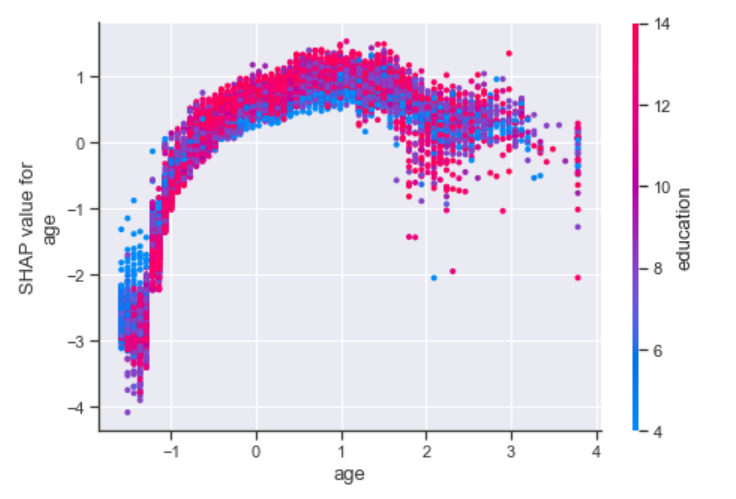
\includegraphics[scale = 0.7]{shap-dependence-plot.png}
            \begin{itemize}[leftmargin = 2em]
                \item this is a plot for training dataset
                \item we can see that smaller age leads to smaller SHAP value (means less likely to predict the positive class)
                \item we can also notice that non-linear relationship, so middle-aged people are more likely to get predicted positive class rather than very young and very old people 
            \end{itemize}
            \item summary plots: shows overall impact for all features\\
            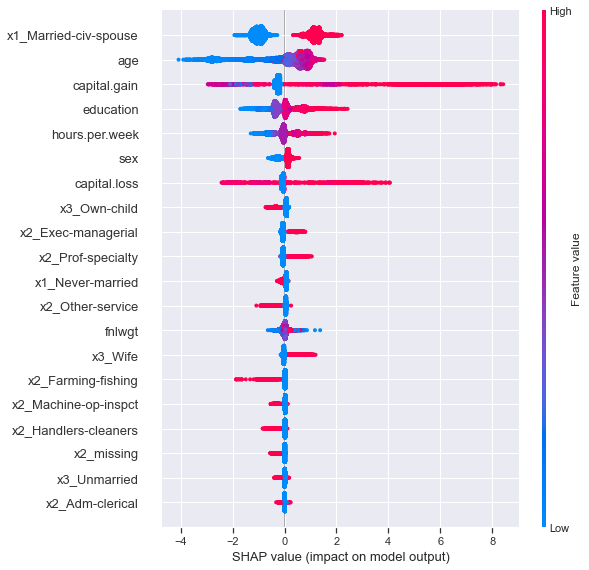
\includegraphics[scale = 0.6]{shap-summary-plots.png}
            \begin{itemize}
                \item colours here represent SHAP value (red being high SHAP value)
                \item so we can see that higher capital gain means a bigger SHAP value 
            \end{itemize}
            \item force plot: how are the features pushing/pulling away from the expected (avg) \ul{for one example} (used to justify/explain the model's prediction)\\
            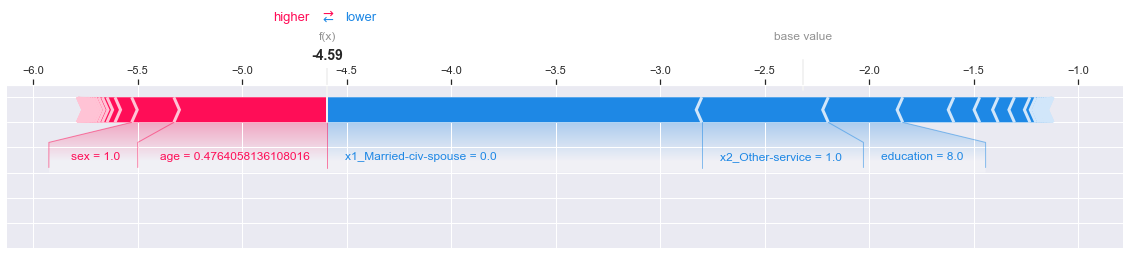
\includegraphics[scale = 0.4]{shap-force-plots.png}
            \begin{itemize}
                \item this was ran on an example that was a negative class (actual target)
                \item see how certain things is pushing it back and forward from the average - i.e absence of spouse is pushing it to be more negative, and more negative means we're more likely to predict the negative class 
            \end{itemize}
        \end{itemize}
    \end{itemize}
\end{itemize}

\newpage

\section*{Chapter 13: Feature Engineering and Feature Selection}
\sectionbookmark{Chapter 13: Feature Engineering and Feature Selection}
\subsection*{Feature Engineering}
\begin{itemize}
    \item \ul{Feature Engineering}: process of transforming raw data into features that better represent underlying problem to the predictive models, resulting in improved model accuracy on unseen data
    \item better features = better models $\rightarrow$ good features should
    \begin{itemize}
        \item capture important aspects of problem
        \item allow learning with few examples
        \item generalize to new scenarios
    \end{itemize}
    \item trade-off between simple vs expressive features
    \begin{itemize}
        \item simple features: overfitting risk is low, but scores might be low
        \item complicated features: scores can be high, but so is overfitting risk 
    \end{itemize}
    \item best features (decided by the feature) is dependent on model you use $\rightarrow$ so there's no concept of universal "best features"
    \item domain specific transformations: there are some natural transformations to do for some domains (i.e image data, sound data, etc) - we'll focus on 
    \begin{itemize}
        \item text data
        \item audio data
    \end{itemize}
    \item common features used in text classification
    \begin{itemize}
        \item bag of words
        \begin{itemize}[leftmargin = 2em]
            \item see above, good for many things
            \item the encoding throws out a lot of things we know about language (i.e assumes word order isn't important)
            \item to improve scores you carry out feature engineering 
        \end{itemize}
        \item N-grams
        \begin{itemize}[leftmargin = 2em]
            \item incorporates more context
            \item likes BOW but takes in a contiguous sequence of $n$-words in test
            \item do this by passing \lstinline{ngram_range} into \lstinline{CountVectorizer}
            \item increasing \lstinline{ngram_range} means more likely to overfit 
        \end{itemize}
        \item Part-of-speech (POS) features
        \begin{itemize}[leftmargin = 2em]
            \item a kind of syntactic category that tells you some of the grammatical property of a word 
            \item it attaches a POS tag to each word
            \item we often use pre-trained models to extract POS information (i.e \lstinline{SpaCy} or \lstinline{ntlk}) $\rightarrow$ can even interpret emojis
        \end{itemize}
    \end{itemize}
    \item classify music style from audio files 
    \begin{itemize}
        \item we'll use \lstinline{librosa} for feature engineering of audio files
        \item much better results with domain-specific features
    \end{itemize}
\end{itemize}

\subsection*{Feature Selection}
\begin{itemize}
    \item reasons for feature selection
    \begin{itemize}
        \item interpetability: less features are more interpretable 
        \item computation: faster fit/predict with fewer columns
        \item data collection: cheaper to collect with fewer columns
        \item fundamental trade-off: can reduce overfitting by removing useless features 
    \end{itemize}
    \item methods for feature selection
    \begin{itemize}
        \item use domain knowledge to discard features
        \item automatic methods: 
        \begin{itemize}[leftmargin = 2em]
            \item model-based selection
            \item recursive feature-elemination
            \item forward selection
        \end{itemize}
    \end{itemize}
    \item \ul{model-based selection}: use a supervised machine learning model to get feature importance, pick ones that we deem are important, then finally pass the remain features into our final estimator 
    \begin{itemize}
        \item model used for feature selection can be different from one used in final estimator 
        \item use \lstinline{SelectFromModel} transformer $\rightarrow$ can pass into a pipeline (usually after transformer steps
        \item it selects from features which have feature importance greater than provided threshold (so pick features with \lstinline{predict_proba} score greater than a certain threshold)
    \end{itemize}
    \item \ul{recursive feature elimination (RFE)}:
    \begin{itemize}
        \item build a series of model, at each iteration, discard the least important feature according to the model 
        \item it's like model-based selection many times $\rightarrow$ computationally expensive 
        \item basic idea: fit model $\rightarrow$ find least important feature (just 1 each time) $\rightarrow$ remove $\rightarrow$ iterate
        \item you will need to decide on $k$ - number of features to select
        \item you can use CV (namely \lstinline{RFECV} to use cross-validation to select number of features) $\rightarrow$ this is insanely slow (bc it's CV within CV)
    \end{itemize}
    \item \ul{Search and Score}:
    \begin{itemize}
        \item define a scoring function $f(S)$ that measures quality of set of features $S$, now search for best set of features $S$ (where $S$ is can be any combination of the features) - stop when adding/removing a feature doensn't improve the score
        \item pick the $S$ with the best score
        \item let number of features $= n$, there are $2^n$ combinations that you need to try out
    \end{itemize}
    \item \ul{Forward or Backwards Selection} (aka wrapper methods):
    \begin{itemize}
        \item shrink or grow feature set by removing/adding one feature at a time 
        \item makes the decision based on whether adding/removing feature improves CV scores or not (below is example of forward selection)\\
        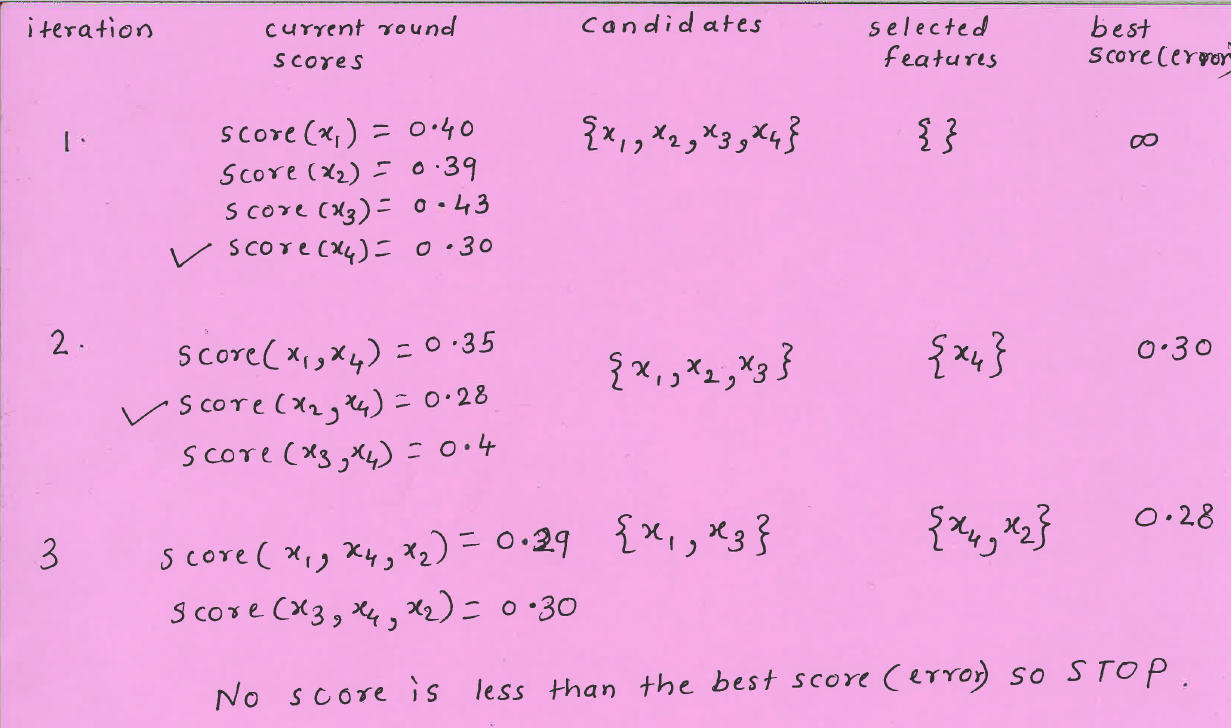
\includegraphics[scale = 0.3]{forward-selection.png}
    \end{itemize}
    \item \ul{warning about feature selection}
    \begin{itemize}
        \item feature's relevance is only defined in context of other features (i.e adding/removing features can make features relevant/irrelevant 
        \begin{itemize}[leftmargin = 2em]
            \item simple association-based feature selection approaches do not take into account the interaction between features
        \end{itemize}
        \item if features can be predicted from other features, you cannot know which one to pick 
        \item relevance for features does not have a casual relationship 
    \end{itemize}
\end{itemize}

\section*{Chapter 14: Clustering}
\sectionbookmark{Chapter 14: Clustering}
\begin{itemize}
    \item \ul{clustering}: task of partitioning dataset into groups called clusters $\rightarrow$ is unsupervised learning 
    \begin{itemize}
        \item if you have access to labeled training data - you're in "supervised" learning 
        \item for unsupervised, training data consists of observations ($X$) with no corresponding targets
        \item we can learn without targets but it'll be focused on finding the underlying structure of input 
    \end{itemize}
    \item most intuitive way to get useful information from unlabeled data is to group similar examples together to gain insights
    \item in clustering, meaningful groups are dependent on the application $\rightarrow$ makes it hard to measure quality of clustering algorithm
    \item similarity and distance
    \begin{itemize}
        \item clustering is based on the notion of similarity or distance between points 
        \item we'll be using Euclidean distance just like kNN
    \end{itemize}
    \item \ul{K-Means clustering}
    \begin{itemize}
        \item input: \lstinline{X} - a set of data points and \lstinline{k} (or \lstinline{n_clusters}) - number of clusters we want
        \item output: $k$ clusters (groups) of data points 
        \item main idea: represent each cluster by its cluster center and assign a cluster membership to each data point
        \item hyperparameter: \lstinline{n_clusters} - though we can't do CV to determine K, we need to do something else, see below 
    \end{itemize}
    \item K-Means algorithm:
        \begin{itemize}
            \item input: data points X and the number of clusters $k$
            \item initialization: $k$ initial centers for the clusters
            \item iterative process: 
            \begin{itemize}[leftmargin = 2em]
                \item assign each example to closest center 
                \item estimate new centers as average of observations in a cluster 
                \item do this until centers stop changing or maximum iteration reached 
                \item when centers stop moving - it means that the algorithm has converged $\longrightarrow$ \textbf{K-Means always converge (not always to optimal solution)}
            \end{itemize}
            \item \ul{\textbf{because k-Means depends on stochastic initialization of the initial cluster centers - how they're initialized can affect the results big time}}
            \item note that \ul{K-mean is really bad at identifying complex shapes} (see lecture 15 K-means recap)
            \item \ul{every point get assigned to a cluster} (even if it's bad)
        \end{itemize}
    \item Hyperparameter tuning 
    \begin{itemize}
        \item Elbow Method: looks at sum of intra-cluster distances (aka inertia)
        \begin{align*}
            \sum_{P_i \in C_1}  distance(P_i, C_1)^2 + \sum_{P_i \in C_2}  distance(P_i, C_2)^2 + \sum_{P_i \in C_3} distance(P_i, C_3)^2
        \end{align*}
        $C_i$ are the cluster centers ~~~~~~~~~~$P_i$s are the points in that cluster \\
        Distance is the euclidean distance \\
        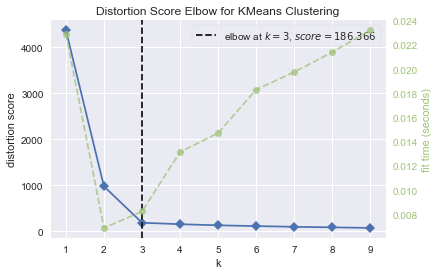
\includegraphics[scale = 0.7]{elbow-plot.png}
        \begin{itemize}[leftmargin = 2em]
            \item \ul{inertia decreases as K increases} 
            \item we want inertia to be small (though picking k to be too big would mean our model is useless)
            \item do elbow plot and pick the $k$ with big improvement from $k-1$ but not so much improvement in going to $k+1$
            \item can use \lstinline{yellowbrick} to make easy elbow plots
        \end{itemize}
        \item Silhouette Method: calculated using the \textbf{mean intra-cluster distance} ($a$) and the \textbf{mean nearest-cluster distnace} ($b$) for each sample 
        \begin{itemize}[leftmargin = 2em]
            \item mean intra-cluster distance ($a$):
            \item mean nearest-cluster distance ($b$):
            \item silhouette distance for a sample:
            \begin{align*}
                \frac{b-a}{max(a,b)}
            \end{align*}
            \item best value is 1, worst is -1 (samples has been assigned to wrong cluster)
            \item value near 0 means overlapping clusters 
            \item the overall Silhouette score is average of Silhouette scores for all samples 
            \item we can plot Silhouette scores for each cluster sample \\
            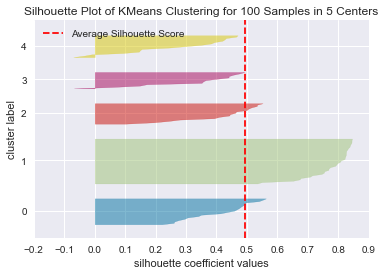
\includegraphics[scale = 0.7]{silhouette-plot.png}
            \begin{itemize}
                \item size of silhouette shows number of data in the samples (so show imbalance of data points in clusters)
                \item higher value indicate well separated clusters 
                \item thickness of silhouette indicates cluster size
                \item shape of each silhhouette indicates the "goodness" for points in each cluster
                \item length (area) of each silhouette shows goodness of each cluster
                \item slower dropoff (more rectangular) indicates more points are "happy" in their clusters
            \end{itemize}
            \item larger values of average Silhouette scores are better 
        \end{itemize}
    \end{itemize}
    \item \textbf{\ul{preprocessing methods like scaling and imputation are unsupervised methods}}
\end{itemize}

\newpage

\section*{Chapter 15: DBSCAN and Recommender Systems}
\sectionbookmark{Chapter 15: DBSCAN and Recommender Systems}
\subsection*{DBSCAN}
\begin{itemize}
    \item DBSCAN: Density-Based Spatial Clustering Applications with Noise
    \begin{itemize}
        \item it's based on the idea that clusters form dense regions in the data - so it works to identify "crowded" regions 
        \item can address some limitations we saw like:
        \begin{itemize}[leftmargin = 2em]
            \item does not require user to specify number of clusters in advance
            \item can identify points that are not part of any clusters
            \item \ul{can capture clusters of complex shape}
        \end{itemize}
        \item hyperparameters
        \begin{itemize}[leftmargin = 2em]
            \item \lstinline{eps}: determines what it means for points to be "close"
            \item \lstinline{min_samples}: determines number of neighbouring points required to consider a point to be a part of a cluster
        \end{itemize}
        \item effects of hyperparameters
        \begin{itemize}[leftmargin = 2em]
            \item small \lstinline{eps} means that if there's just one data point, it'll be considered a cluster (we will get a lot of noise points)
            \item large \lstinline{min_samples} means that we might consider everything to be a cluster 
            \item we want something in between (thus we will have to tune the hyperparameters)
        \end{itemize}
        \item \ul{we cannot call predict} (DBSCAN only clusters clusters point you have, not new/test points)
    \end{itemize}
    \item DBSCAN algorithm: is iterative
    \begin{itemize}[leftmargin = 2em]
        \item start with random point
        \item check if that point is part of crowded area (if there's enough neighbours)
        \item give some colour to that point if so, spread that colour to all its neighbours
        \item do the same for all its neighbours 
        \item when you run out of points, you pick a new random point \textbf{that hasn't been visited before}
        \item rinse and repeat
    \end{itemize}
    \item hyperparameter tuning: cannot use elbow method, \ul{but can use silhouette method}
    \item weaknesses: doesn't do very well when we have clusters of different densities (K Means can handle these cases quite easily)
\end{itemize}
\subsection*{Recommender Systems}
\begin{itemize}
    \item recommender system: a system that recommends a particular product/service to users that they're likely to consume
    \item main approaches:
    \begin{itemize}
        \item collaborative filtering (most popular)
        \begin{itemize}[leftmargin = 2em]
            \item unsupervised learning
            \item we have labels $y_{ij}$ (ratings of user $i$ for item $j$) aka utility matrix
            \item we learn the features
        \end{itemize}
        \item content-based recommenders
        \begin{itemize}[leftmargin = 2em]
            \item supervised learning
            \item extract features $x_i$ of users and/or items and building a model to predict rating $y_i$ given $x_i$
            \item apply model to predict for new users/items
        \end{itemize}
        \item hybrid: mixed of both above
    \end{itemize}
    \item Collaborative Filtering
    \begin{itemize}
        \item given a utility matrix of $N$ users and $M$ items (which is usually sprase), we want to complete it (predict the missing values in the matrix \\
        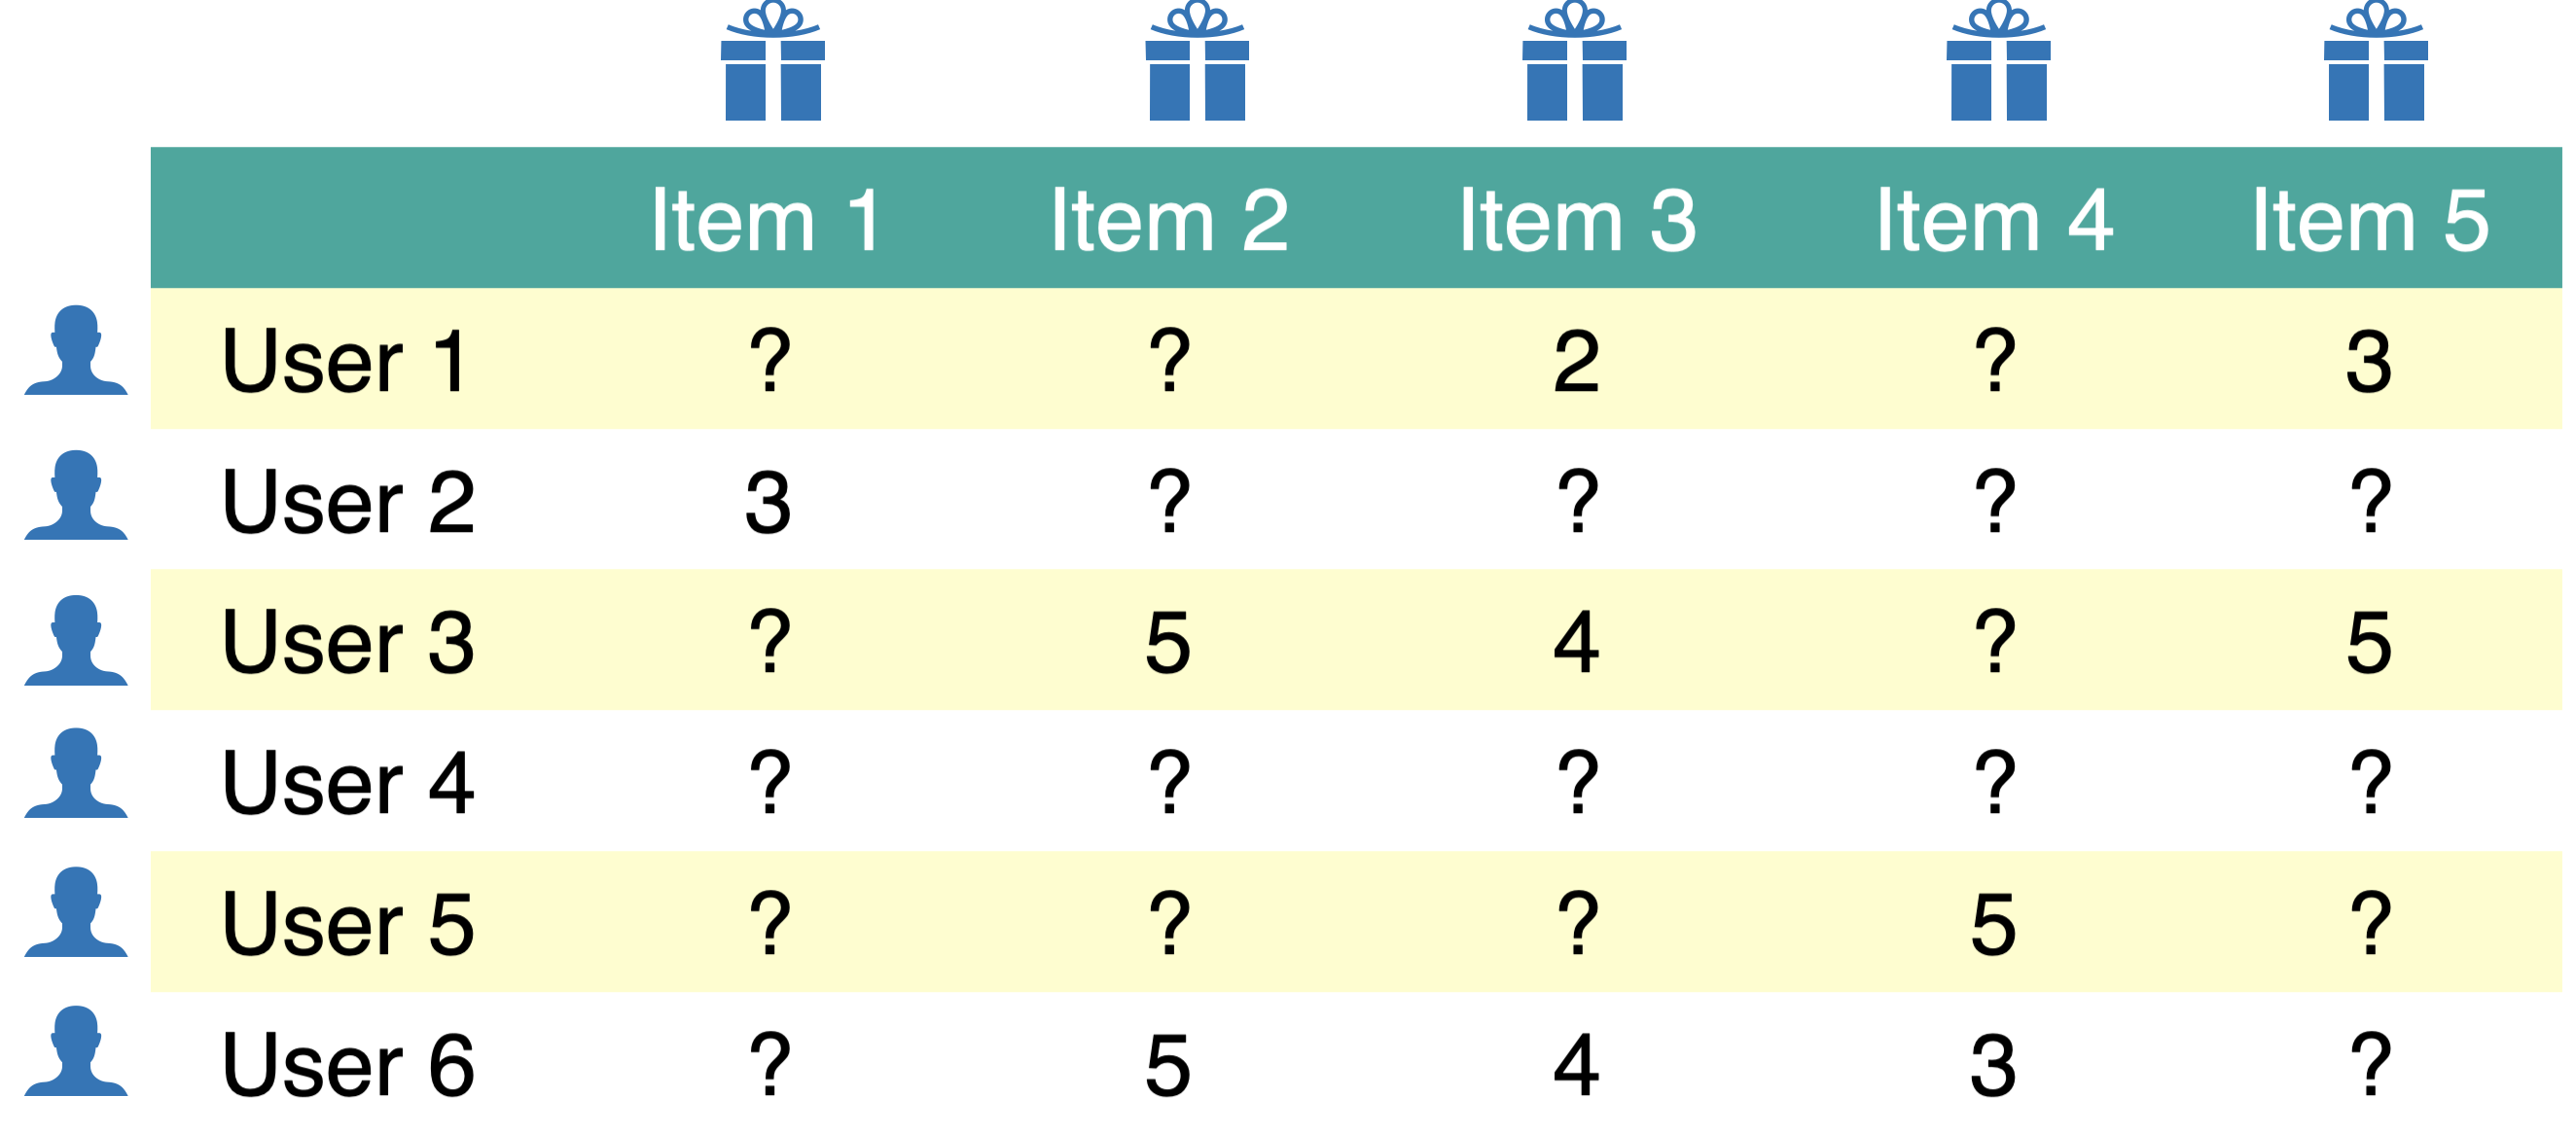
\includegraphics[scale = 0.3]{utility-matrix.png}
        \item we'll use an algorithm called \lstinline{SVD} from package \lstinline{surprise}
    \end{itemize}
    \item Evaluation and Data Splitting 
    \begin{itemize}
        \item though there's no notion of "accurate" recommendations, we need a way to evaluate our predictions to compare between methods
        \item we'll split the data and evaluate our predictions as follows: split the ratings into train and validation sets (not split the utility matrix) \textbf{then} create utility matrix for train and validation splits
        \item during training we assume that we do not have access to some of the available ratings. We predict these ratings and evaluate them against ratings in the validation set.
        \item Important notes:
        \begin{itemize}[leftmargin = 2em]
            \item training matrix is of shape N by M but only has ratings from \lstinline{X_train} and all other ratings missing
            \item validation matrix is als oof shape N by M but only has ratings from \lstinline{X_valid} and all other ratings missing
        \end{itemize}
        \item we can calculate errors between actual ratings and predicted ratings with any metrics of our choice (common is MSE and RMSE)
    \end{itemize}
    \item baselines: there are a couple of baseline approaches
    \begin{itemize}
        \item global average baselines: predict all missing value as the global average rating
        \item k-NN imputation: impute missing values using mean value from k nearest neighbours found in the dataset
    \end{itemize}
    \item to see how to actually do collaborative filtering, see "Collaborative filtering $\rightarrow$ Rating prediction using the surprise package"
    \item Cross Validation: we can carry out cross validation and grid search using \lstinline{surprise} package
    \item \ul{Content Based Filtering}: 
    \begin{itemize}
        \item supervised machine learning approach
        \item in collaborative filtering we assumed that we only have ratings data, but usually there is some information on items and users available. 
        \item examples
        \begin{itemize}
            \item Netflix can describe movies as action, romance, comedy, documentaries. 
            \item Amazon could describe books according to topics: math, languages, history. 
        \end{itemize}
        \item we can use these information to make a utility matrix
        % \item it would be reasonable to impute missing values in the utility matrix by taking the average of the ratings given to an item by similar users
    \end{itemize}
\end{itemize}

\section*{Chapter 16: NLP} 
\sectionbookmark{Chapter 16: NLP} 
\subsection*{Word Embeddings}
\begin{itemize}
    \item word embeddings (representation): idea is to represent word meaning so that similar words are close together
    \begin{itemize}
        \item so far we've been talking about sentence/document representation (BOW)
        \item though word representation can't be used in text classification tasks like sentiment analysis using traditional ML models, they are useful for advanced ML models like neural networks 
        \item word embeddings allow use to solve meaning-related problems (i.e what is the meaning of "gloves") or which find relationships between words (which words are similar, which ones have positive/negative connotation)
    \end{itemize}
    \item how to represent words
    \begin{itemize}
        \item we will need a representation that captures relationships between worse 
        \item we'll be looking at 2 such reprsentations
        \begin{itemize}[leftmargin = 2em]
            \item sparse representation with \ul{\textbf{term-term co-occurrence matrix}}
            \item dense representation with \ul{\textbf{Word2Vec}}
            \item both are based on \textbf{distributional hypothesis} and \textbf{vector space model}
        \end{itemize}
    \end{itemize}
    \item Vector Space model: model meaning of a word by placing it into a vector space 
    \begin{itemize}
        \item idea is to create embeddings of words so that distances among words in the vector space indicate relationship between them \\
        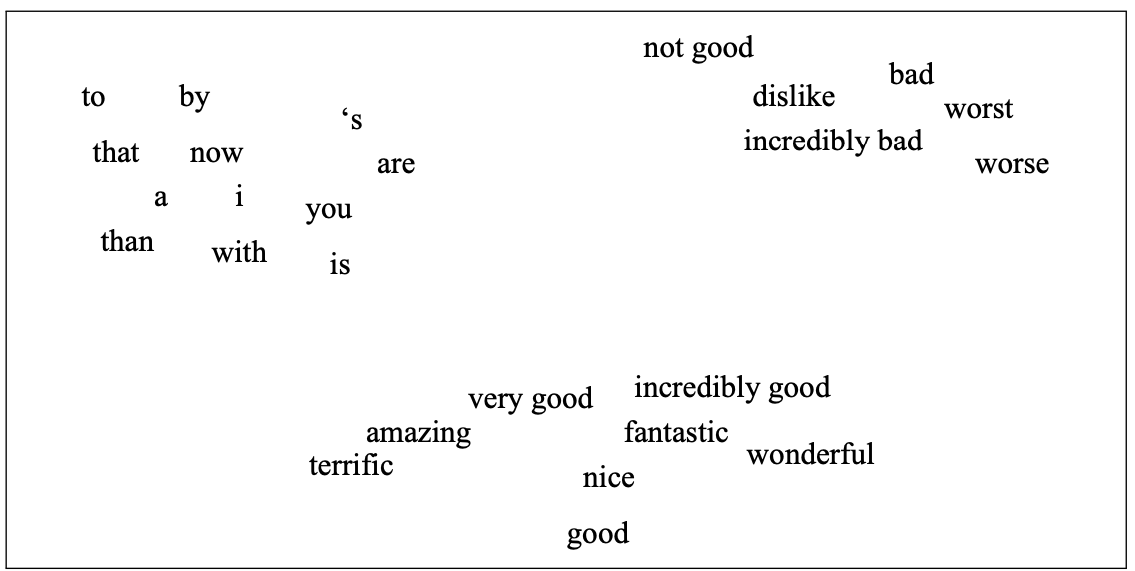
\includegraphics[scale = 0.3]{vector-space.png}
    \end{itemize} 
    \newpage 
    \item Term-Term Co-Occurrence Model 
    \begin{itemize}
        \item same idea as bag of words but for texts appearances instead
        \item you go through large corpus of text, keep count of all words that appear in context of each word (within a window) \\ 
        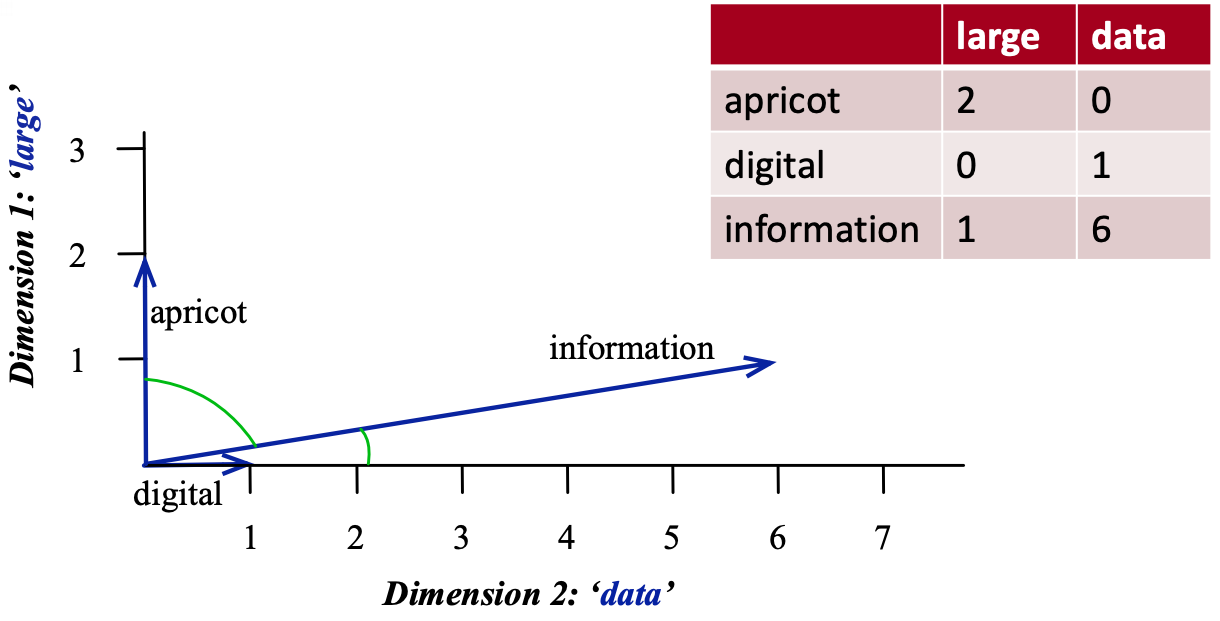
\includegraphics[scale = 0.3]{term-term-matrix.png}
        \item you can plot these (large column on the y-axis, and data column on the x-axis, with the words being vectors so apricot would be vector $<2,0>$) 
        \item similarity within words can be calculated using the dot products between vectors (i.e digital $\cdot$ information $= (0 \times 1) + (1 \times 6) = 6 \longrightarrow$ higher the dot product the more similar the words 
        \item similarity can also be captured via cosine similarity
        \item these matrices are usually are long and sparse (most elements are 0)
        \begin{itemize}[leftmargin = 2em]
            \item the alternative is to learn short and dense vectors, these are easier to train with ML models and may generalize better
            \item in practice dense vectors they work much better 
        \end{itemize}
    \end{itemize}
    \item Word2Vec: a family of algorithms to create dense word embeddings 
    \begin{itemize}
        \item create dense representation by using \lstinline{gensim} or \lstinline{spaCy}
        \item you can additionally download pre-trained embeddings that's been trained on huge corpus (like Wikipedia)
        \item with this you can find words most similar to a word of your choice, or find similarity within words, even find analogies (Lecture 16 $\rightarrow$ word representations $\rightarrow$ finding similar words)
        \item Note: there maybe gender/racial stereotypes embedded into the word embeddings
    \end{itemize}
    \item representing documents using word embeddings: how to represent meaning of paragraphs or documents (assuming we have reasonable representation of words)
    \begin{itemize}
        \item averaging embeddings
        \item concatenating embeddings
    \end{itemize}
    \item average embeddings: get embedding of each word in the sentence and divide by the number of words
    \begin{itemize}
        \item ex. all empty promises = $[embedding(all) + embedding(empty) + embedding(promise)]/3$
        \item using this, you're able to find similarity between documents as well 
        \item sentiment analysis using average embeddings (as opposed to BOW) reduced overfitting
    \end{itemize}
    \item Sentence Transformer: fancier methods for document representation 
    \begin{itemize}
        \item better score than both BOW and average embedding but much much slower 
    \end{itemize}
\end{itemize}

\subsection*{Topic Modelling}
\begin{itemize}
    \item suppose you have a large collection of documents on a variety of topics - you want to categorize them so it's easy to search - topic modelling gives you ability to summarize major themes in a large collection of documents
    \item topic modelling
    \begin{itemize}
        \item usually solve via unsupervised ML methods
        \item give hyperparameter K, describe the data using K topics
        \item input: 
        \begin{itemize}[leftmargin = 2em]
            \item large collection of documents 
            \item value for the hyperparameter k
        \end{itemize}
        \item output: 
        \begin{itemize}[leftmargin = 2em]
            \item topic-words association: for each topic, what words describe the topic 
            \item document-topics association: for each document, what topics are expressed by the document
        \end{itemize}
        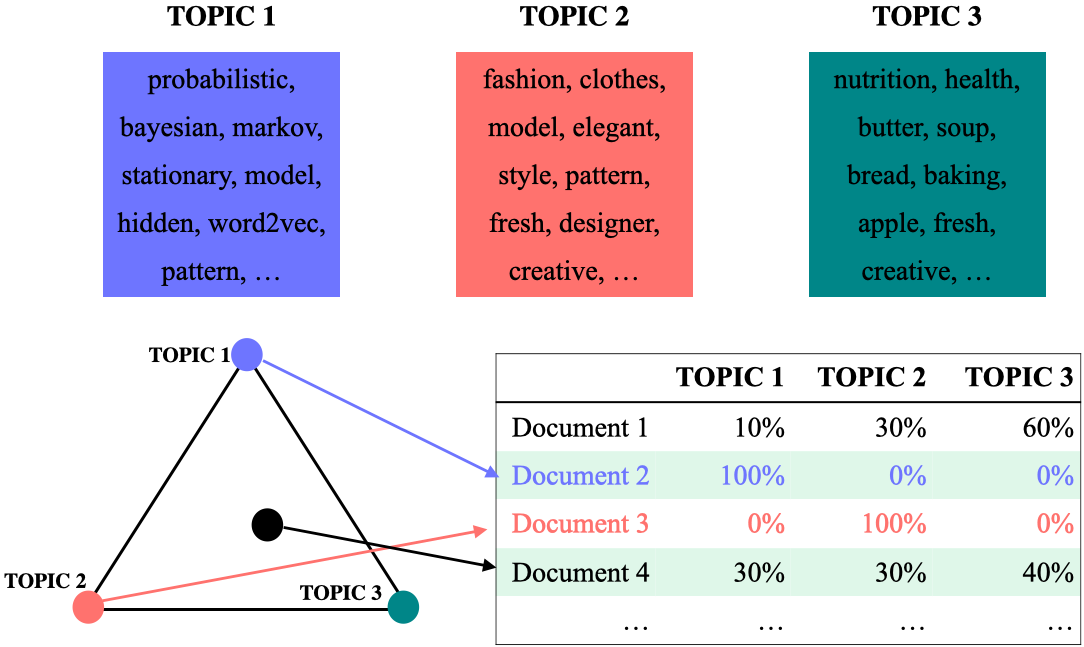
\includegraphics[scale = 0.3]{topic-modelling.png}
    \end{itemize}
    \item we'll be training using an \lstinline{LDA} model
    \item process
    \begin{enumerate}
        \item preprocess your corpus
        \item train LDA using \lstinline{gensim}
        \item interpret your topics 
    \end{enumerate}
\end{itemize}

\subsection*{Basic Text Preprocessing}
\begin{itemize}
    \item we need to do preprocessing because test data is unstructured and messy
    \item tokenization
    \begin{itemize}
        \item sentence segmentation: split text into sentences
        \item word tokenization: split sentences into words
    \end{itemize}
    \item Sentence segmentation
    \begin{itemize}
        \item you can tell python to do segmentation on punctuation (like periods or exclamation marks)
        \begin{itemize}[leftmargin = 2em]
            \item even then, it might be ambigious (at least period is in English - could be Dr. or U.S or decimal)
        \end{itemize}
        \item common way is too use off-the-shelf models for sentence segmentation
        \begin{itemize}[leftmargin = 2em]
            \item using \lstinline{ntlk}
        \end{itemize}
    \end{itemize}
    \item Word tokenization
    \begin{itemize}
        \item what are the boundaries we decide for something to be a word (is white space enough) - the process of identifying word boundaries is known as tokenization
        \item also use off-the-shelf ML models 
        \begin{itemize}[leftmargin = 2em]
            \item also use \lstinline{ntlk}
        \end{itemize}
    \end{itemize}
    \item types and tokens: types are all \textbf{unique} words, tokens are just word counts
    \item punctuation and stopword removal: removing words like "the", "is", "a" and punctuations
    \begin{itemize}
        \item also can be done with \lstinline{ntlk}
    \end{itemize}
    \item Lemmatization: sometimes we want to ignore morphological differences betwen words 
    \begin{itemize}
        \item ex. if your search term is “studying for ML quiz” you might want to include pages containing “tips to study for an ML quiz” or “here is how I studied for my ML quiz”
        \item can be done via \lstinline{ntlk}
    \end{itemize}
    \item Stemming: chops of affixes
    \begin{itemize}
        \item ex.automates, automatic, automation all reduced to automat
        \item can be done via \lstinline{ntlk}
    \end{itemize}
    \item \ul{\textbf{every text processing method we said above can be done in spaCy}}
\end{itemize}

\section*{Chapter 17: Multi-class classification and Computer Vision}
\sectionbookmark{Chapter 17: Multi-class classification and Computer Vision}
\subsection*{Multi-class Classification}
\begin{itemize}
    \item sometimes we need to do classification with more than 2 classes 
    \item many linear classification models don't extend naturally to the multi-class case, so we'll need some techniques to get around this 
    \item 2 kinds of approaches
    \begin{itemize}
        \item one-vs-rest approach (OVR)
        \item one-vs-one approach (OVO) 
    \end{itemize}
    \item \ul{One vs. Rest}
    \begin{itemize}
        \item learn a binary model for each class which tries to separate that class from all other class 
        \begin{itemize}[leftmargin = 2em]
            \item ex. you have 3 class, you'd try out: \\
            1 vs \{2,3\} (so either class 1 or the other)\\
            2 vs \{1,3\} (either class 2 or the other)\\
            3 vs \{1, 2\} (either class 3 or the other)
        \end{itemize}
        \item if you have $k$ classes, it'll train $k$ binary classifiers, one for each class
        \item it'll be train on imbalanced datasets containing all examples
        \item given test point, get scores from all binary classifiers (e.g. raw score for LR) $\rightarrow$ the classifier which has the highest score, choose the one class from that classifier 
        \begin{itemize}[leftmargin = 2em]
            \item ex. given test point, $LR_{1 \text{ vs } \{2,3\}} = 0.6, LR_{2 \text{ vs } \{1,3\}} = 0.5, LR_{3 \text{ vs } \{1,2\}} = 0.3$, predict class 1
        \end{itemize}
        \item since we have $k$ classifier, we will have coefficients and intercept for each of those classifiers (enough to make $k$ lines) $\rightarrow$ you can also get $k$ decision boundaries which makes it a little easier to predict new points
        \end{itemize}
        \item \ul{One vs. One Approach}
        \begin{itemize}
            \item build a binary model for each pair of classes 
            \begin{itemize}[leftmargin = 2em]
                \item ex. 1 vs 2, 1 vs 3, 2 vs 3
            \end{itemize}
            \item will train $\dfrac{n(n-1)}{2}$ binary classifiers 
            \item trained on relatively balanced subsets (will ignore the other classes - for example, for the 1 vs 2 classifier, it will ignore all points of class 3)
            \item predictions: apply all classifiers on test example $\rightarrow$ count how often each class was predicted $\rightarrow$ predict the class with the most votes
        \end{itemize}
        \item OVO takes more time than OVR
        \item unlikely you will need to use them because most models have multi-class support
\end{itemize}

\subsection*{Intro to Computer Vision}
\begin{itemize}
    \item computer vision: understanding images/videos, esp using ML/AI (neural network specifically in our case)
    \item neural network: apply a sequence of transformations on your input data 
    \begin{itemize}
        \item involves a series of transformations (layers)
        \item think about it a bit like LR - doing weighted sums, but what makes neural network more powerful than linear models is that we can apply non-linear function to weighted sum for each hidden nodes 
    \end{itemize}
    \item pros of neural network: 
    \begin{itemize}
        \item can learn very complex functions (more/bigger layers = more complex model), you can generally get a model that will not underfit
        \item works well for structured data (i.e 1D sequence - like time series, language; 2D image; 3D image/video)
        \item transfer learning (later) is very useful
    \end{itemize}
    \item cons of neural network:
    \begin{itemize}
        \item require a lot of data
        \item computationally expensive 
        \item have a lot of hyperparameters which are hard to tune 
        \item not very interpretable 
        \item when you call \lstinline{fit}, you are not guaranteed to get the optimal
    \end{itemize}
    \item we can try to use basic ML like LR on tabular image data (squashed into array of numbers that represent numbers - "flattening the image") but our results are garbage 
    \begin{itemize}
        \item flattening the image throws away useful information
    \end{itemize}
    \item transfer learning: use pre-trained (neural network) models (like convolution neural networks - CNN) and fine tune to your need 
\end{itemize}

\section*{Chapter 18: Time Series}
\sectionbookmark{Chapter 18: Time Series}
\begin{itemize}
    \item time series is collection of data points indexed in time order 
    \begin{itemize}
        \item notice when datasets have datetime features
    \end{itemize}
    \item questions we're looking to answer: how many people likely to rent a bike at this station tomorrow at 3pm given everything we know about rentals in the past 
    \item need special way to split time series data
    \begin{itemize}
        \item we don't want to split normally - has chance that we are training on data that came after our "test data" $\rightarrow$ so if we want to forecast, we aren't allowed to know what happened in the future
        \item what we do is treat data before a certain date as training data and everything after as test data
        \begin{itemize}[leftmargin = 2em]
            \item ex. if we have total 248 data points, we'd use the first 184 data (corresponds to first 23 days in a month) as training data and the remaining 64 for the last 8 days as test data
        \end{itemize}
    \end{itemize}
    \item training models
    \begin{itemize}
        \item how to encode time features: using POSIX time 
        \item our prediction test (question above) is a regression task 
        \item \ul{note}: be careful when working with datasets with \textbf{only} time features
        \begin{itemize}[leftmargin = 2em]
            \item \textbf{\ul{tree-based models cannot extrapolate to feature ranges outside the training data}} (see lecture 18 $\rightarrow$ training models)
        \end{itemize}
    \end{itemize}
    \item feature engineering for date/time columns: 
    \begin{itemize}
        \item if our index is of the special type \lstinline{DateTimeIndex} - we can extract a lot of interesting from it, like: 
        \begin{itemize}[leftmargin = 2em]
            \item get month names for each example
            \item get days of the week
            \item get day of the week
            \item hours of the day
        \end{itemize}
        \item just by using time of the day as our feature column we can get better results
        \item we can get even better results by adding a day of week feature as well 
    \end{itemize}
    \item trying \lstinline{Ridge} on data 
    \begin{itemize}
        \item Ridge performs a bit poorly on both training and testing data (not able to pick up periodic pattern)
        \item reason is because we encoded time of day as integers and linear functions and only learn a linear function of the time of day
        \item turning hour and day feature into categorical values really helps
        \item even better if you apply \lstinline{PolynomialFeatures} transformer 
        \item looking at coefficients learned by Ridge useful to predict what time is the most busy 
    \end{itemize}
    \item Cross Validation:
    \begin{itemize}
        \item again, problem with splitting training data into training and validation set
        \item use \lstinline{TimeSeriesSplit} for time series data
    \end{itemize}
    \item can turn string Dates columns into \lstinline{DateTimeIndex} by using pandas' \lstinline{to_datetime()} function
    \item pretty intuitive example using Australia rainfall in Lecture 18 
    \item lag-based features: 
    \begin{itemize}
        \item sometimes there's temporal dependence: observations closer in time tend to be correlated 
        \begin{itemize}[leftmargin = 2em]
            \item ex. what if tomorrow's rain fall is related to yesterday's features, or the day before
            \item this is particularly when the change from one week to another isn't exactly drastic (i.e if next week's avocado price is slightly different from this week then lagged features are a good idea, however, if they fluctate a lot then it's not a good idea)
            \item this is called a lagged (or shift feature)
        \end{itemize}
        \item use pandas' \lstinline{shift} function $\rightarrow$ basically add a lagged feature columns (i.e lagged rainfall feature for day 2 is rainfall feature from day 1)
    \end{itemize}
    \item forecasting further into the future (i.e predict rainfall 7 days into the future)
    \begin{enumerate} 
        \item train a model for each of the days (one for tomorrow, one for the day after, etc) and we can build these datasets (because we have historical data - of course, as the days into the future gets bigger, the dataset gets smaller)
        \item use multi-output model (not in scope of class)
        \item use one model and sequentially predict using for loop (use our predictions as truths and iterate through)
    \end{enumerate}
    \item trends: rely on having a continuous target
    \begin{itemize}
        \item in our example, we used only lag features (ex. sales, sales-1, sales-3, sales 4, ....)
        \item if you have a \lstinline{DaySince} feature and use Linear Regression on it, the coefficient learned will predict unlimited growth forever if it's positive $\rightarrow$ this is your trend 
        \item if you use Random Forest, we'll be doing splits from the training sets (i.e if \lstinline{DaySince} > 9100, do this) and thus there will be no splits for later time points because there's no training data
        \begin{itemize}[leftmargin = 2em]
            \item \textbf{\ul{tree-based models cannot model trend}}
        \end{itemize}
    \end{itemize}
\end{itemize}

\section*{Chapter 19: Survival Analysis}
\sectionbookmark{Chapter 19: Survival Analysis}
\begin{itemize}
    \item useful for problems like the "customer churn" datasets and incoroporating the time feature
    \item when we did binary classification (churn vs not churn), we're missing out on the time aspect - we can't say how long a customer will stay, or how likely they'll stay based on how long they've been with the company 
    \item time to event
    \begin{itemize}
        \item sometimes you want to analyze the time till an event happens (ex. time until a piece of equipment breaks) 
        \item so in our churn, instead of predicting churn or not churn, it's more useful to when the customer is likely to churn 
    \end{itemize}
    \item censoring: when a patient is censored we don’t know the true survival time for that patient
    \begin{itemize}
        \item ex. if we're predicting a tenure of a customer, but we don't know the actual tenure times for tuples where \lstinline{churn = no} (because, well, their tenure hasn't ended yet $\rightarrow$ this is right-censoring)
        \item this is a problem $\rightarrow$ means that we don't have correct target values to train/test model
        \item approach to solve
        \begin{enumerate}[leftmargin = 2em]
            \item only consider examples where \lstinline{churn = "yes"}
            \begin{itemize}[leftmargin = 1.5em]
                \item on average, our predicted tenure time will be underestimates because we are ignoring currently subscribed (unchurned customers)
                \item our dataset is a biased samples of those who churned during data collection time
            \end{itemize}
            \item assume everyone churns right now
            \begin{itemize}[leftmargin = 1.5em]
                \item in other words, use the original dataset
                \item our prediction will again be underestimates, because for those still subscribed, we recorded a shorter total tenure time than reality - because they will keep going for some amount of time
                \item survival analysis: the proper way to deal with this
            \end{itemize}
        \end{enumerate}
    \end{itemize}
    \item survival analysis: use the \lstinline{lifelines} package 
    \newpage 
    \item Kaplan-Meier survival curve: part of the \lstinline{lifelines} package
    \begin{itemize}
        \item for the model, in our example, we only use 2 features - tenure and churn 
        \item we get this curve \\
        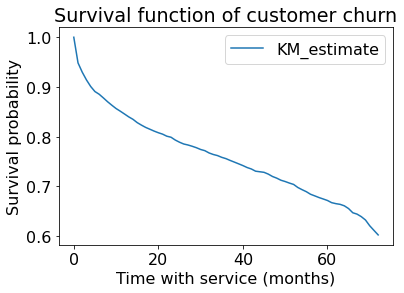
\includegraphics[scale = 0.55]{km-curve.png}
        \item the plot is telling the probability of survival over time 
        \begin{itemize}[leftmargin = 2em]
            \item ex. after 20 months, the probability of survival is about 0.8
            \item steep drop in the beginning that people tend to leave early on 
        \end{itemize}
        \item you can create K-M curve for different subgroups (i.e seniors citizens) and we can see that senior citizens tends to churn more quickly than others  \\
        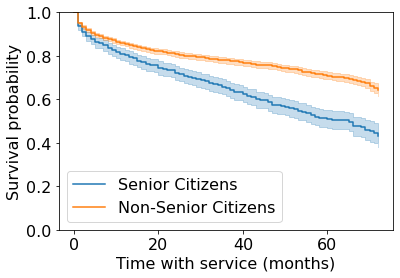
\includegraphics[scale = 0.55]{km-curve-2.png}
    \end{itemize}
    \item Cox proportional hazards model 
    \begin{itemize}
        \item incorporates other features into the model, produces similar survival curve
        \item Cox proportional hazards model is a commonly used model that allows us to interpret how features influence a censored tenure/duration (a bit like linear regression for survival analysis - we'll get coefficient for each feature but it'll tell us how it influences survival)
        \item blah blah we run it on our model, get the coeffiennts and \lstinline{Contract_Month-to-Month = 0.812874} and \lstinline{Contract_Two year = -0.776425} so this means that \ul{month-to-month leads to more churn} while two-year contracts leads to less churn $\rightarrow$ so negative is actually good for companies
        \item \textbf{Cox proportional hazards model assumes the effect of a feature is the same for all customers and over all time}
        \item we can get the survival curve as well, ket's look at the different Monthly Charges, from this, we see that the bigger your bill, the less likely you are to churn (higher survival rate) so we should expect a negative coefficient \\
        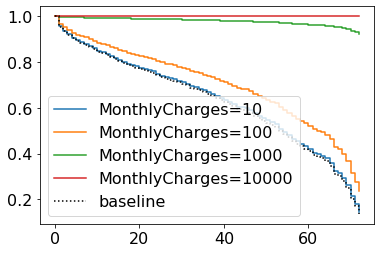
\includegraphics[scale = 0.55]{cph-plot.png}
    \end{itemize}
    \item predictions: we can use survival analysis to make predictions 
    \begin{itemize}
        \item we can predict how long each non-churned customer is likely to stay according to the model \ul{assuming that they just joined right now} (so we drop the churn column)
        \item you can condition the function on certain things (i.e how long they're gonna stay given they've been here 20 months - instead of assuming starting now)
        \item thus, we can then do a graph of how long each non-churned customer is likely to stay according to the model assuming they've been here for the tenure time 
    \end{itemize} 
    \newpage
    \item evaluations: by default returns "partial log-likelihood"
    \begin{itemize}
        \item however, concordance index (c-index) is more interpretable
        \begin{itemize}[leftmargin = 2em]
            \item 0.5 is expected results from random predictions
            \item 1.0 is perfect concordance 
            \item 0.0 perfect anti-concordance (multiply results with -1 to get 1 - so predicting opposite)
        \end{itemize}
    \end{itemize}
\end{itemize}

\section*{Chapter 20: Ethics}
\sectionbookmark{Chapter 20: Ethics}
\begin{itemize} 
\item here, we use the fraud banks example and observe the confusion matrix between the two (it's male only on the left and female only on the right)
     \begin{figure}[!h]
        \centering
        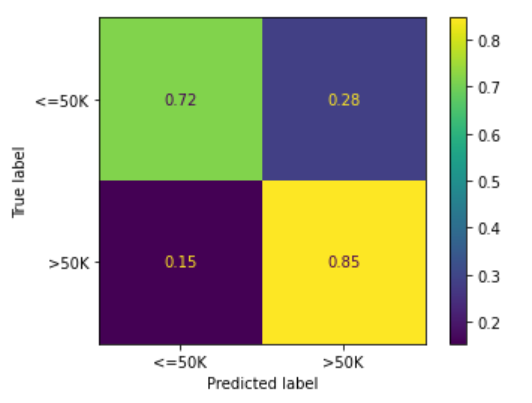
\includegraphics[scale = 0.85]{cfm-male.png} 
        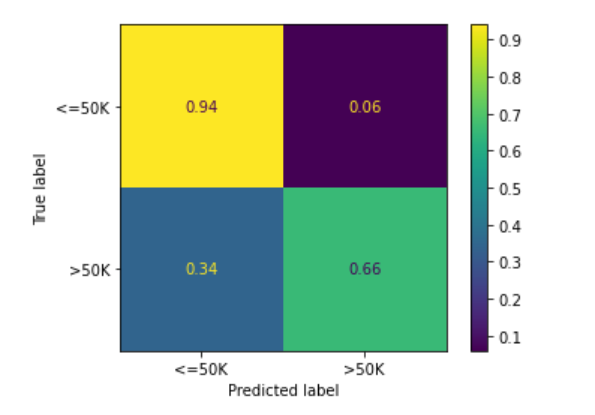
\includegraphics[scale = 0.75]{cfm-female.png}
        \label{fig:my_label}    
    \end{figure}
    \begin{itemize}
        \item notice that there are more false negative for females, so even though they make more than 50k, the model assumes otherwise
        \item also notice that there are more false positives for males
        \item we see that $\text{accuracy male} = 0.756$ while accuracy female $= 0.910$ $\rightarrow$ could be explained by class imbalance 
        \item if we do value counts we see that there's a bigger class imbalance for females [0.90, 0.10] vs males [0.70, 0.30]
        \item consequence: if you're just looking at predicted income to decide to approve loans or not, male has more chance of getting loans approved
    \end{itemize}
\item \ul{statistical parity} suggests that the proportion of each segment of a protected class (e.g. sex) should receive the positive outcome at equal rates
\begin{itemize}[leftmargin = 2em]
    \item ex. number of loans approved for female should be equal to male
\end{itemize}
\item \ul{equal opportunity} suggests that each group should get positive outcomes at equal rates (assuming they qualify for it) 
\begin{itemize}
    \item \ul{true positive rate (TPR or recall) of both groups should be equal} $\rightarrow$ should look at recall
    \item we see that recall male $= 0.847$ and recall female $= 0.657$
    \item so we can see that we're not giving equal opportunity to men and women (men gets approve more) 
    \item \ul{vastly different recall scores indicate that we're not giving equal opportunity to both groups}
\end{itemize}
\item moreover, banks usually want to approve as many qualified people as possible (true positive), but also to avoid approving unqualified application (false positive) so we should look at false positive rate (FPR)
\begin{itemize}
    \item we get FPR male $= 0.285$ and FPR female $= 0.060$
    \item so we're getting a lot more false positives for men, so we should also take a look at FPR between groups
\end{itemize}
\end{itemize}

\section*{Chapter 21: Communications}
\sectionbookmark{Chapter 21: Communications}
\begin{itemize}
    \item we want to be confident when we're right, but hesitant when we're wrong
    \begin{itemize}
        \item use credence (the bolded parts below)
        \item if Toronto has the highest cost of living and our model predicted otherwise, we want to express hesitancy
        \begin{itemize}[leftmargin= 2em]
            \item ex. Vancouver has the highest cost of living in Canada. \textbf{I am 55\% sure of this}
        \end{itemize}
    \end{itemize}
    \item \ul{loss functions}: when you call \lstinline{fit} for \lstinline{LogisticRegression} it has these same preferences 
    \begin{align*}
        \text{correct and confident} > \text{correct and hesitant} > \text{incorrect and hesitant} > \text{incorrect and confident}
    \end{align*}
    \begin{itemize}
        \item sklearn models use a log loss function $\rightarrow$ it's an "error" function, so lower values are better 
        \item \lstinline{fit} tries to minimize this error
        \item so \textbf{in terms of log loss score}
    \end{itemize}
\end{itemize}
\begin{align*}
    loss(\text{correct and confident}) < loss(\text{correct and hesitant}) < loss(\text{incorrect and hesitant}) < loss(\text{incorrect and confident})
\end{align*}

\end{document}
